% TODO:
% 	explain the concept of MIP

%  Add temperature fluctuation at different room based on outdoor temperature..
%  Add full HVAC model and McCormick Model
%  Add example of back-to-back vs. joint model vs. random
%  Add building configuration - say consider building of different type
%  Add related work and non-linear. say hvac non-linear method can be linearised by bla bla hvac linearisation method. Also include related work on hvac using non-linear. Talk about pre-cooling based on meetings
% Future work: say incorporate humidity bla bla bla, refer hassan paper about multilinear term using sequential mccormick, all positive bounds maybe new way of relaxation is possible.

%  The integrated model should achieve higher efficiency in energy reduction by fully exploiting the capability to coordinate through both HVAC control and occupancy scheduling. 

\chapter{Integrating HVAC Control with Occupancy Scheduling}
%\chapter{HVAC-Aware Occupancy Scheduling}
\label{cha:milp}

\section{Introduction}

% TODO:
%  
%  there have been ppl working on occupancy-based HVAC control
% there have been ppl working on energy-aware scheduling
% crystal-cleared about our joint model >> contributions

% One of the main inefficiencies in building management systems is the widespread use of schedule-based control when operating heating, ventilation and air conditioning (HVAC) systems. HVAC systems typically operate on a pre-designed schedule that heats or cools rooms in the building to a set temperature even when rooms are not being used. Occupants, however, influence the thermal behavior of buildings. As a result, using occupancy information for scheduling meetings to occur at specific times and in specific rooms has significant energy savings potential. 

\begin{figure}[bt]
	\centering
		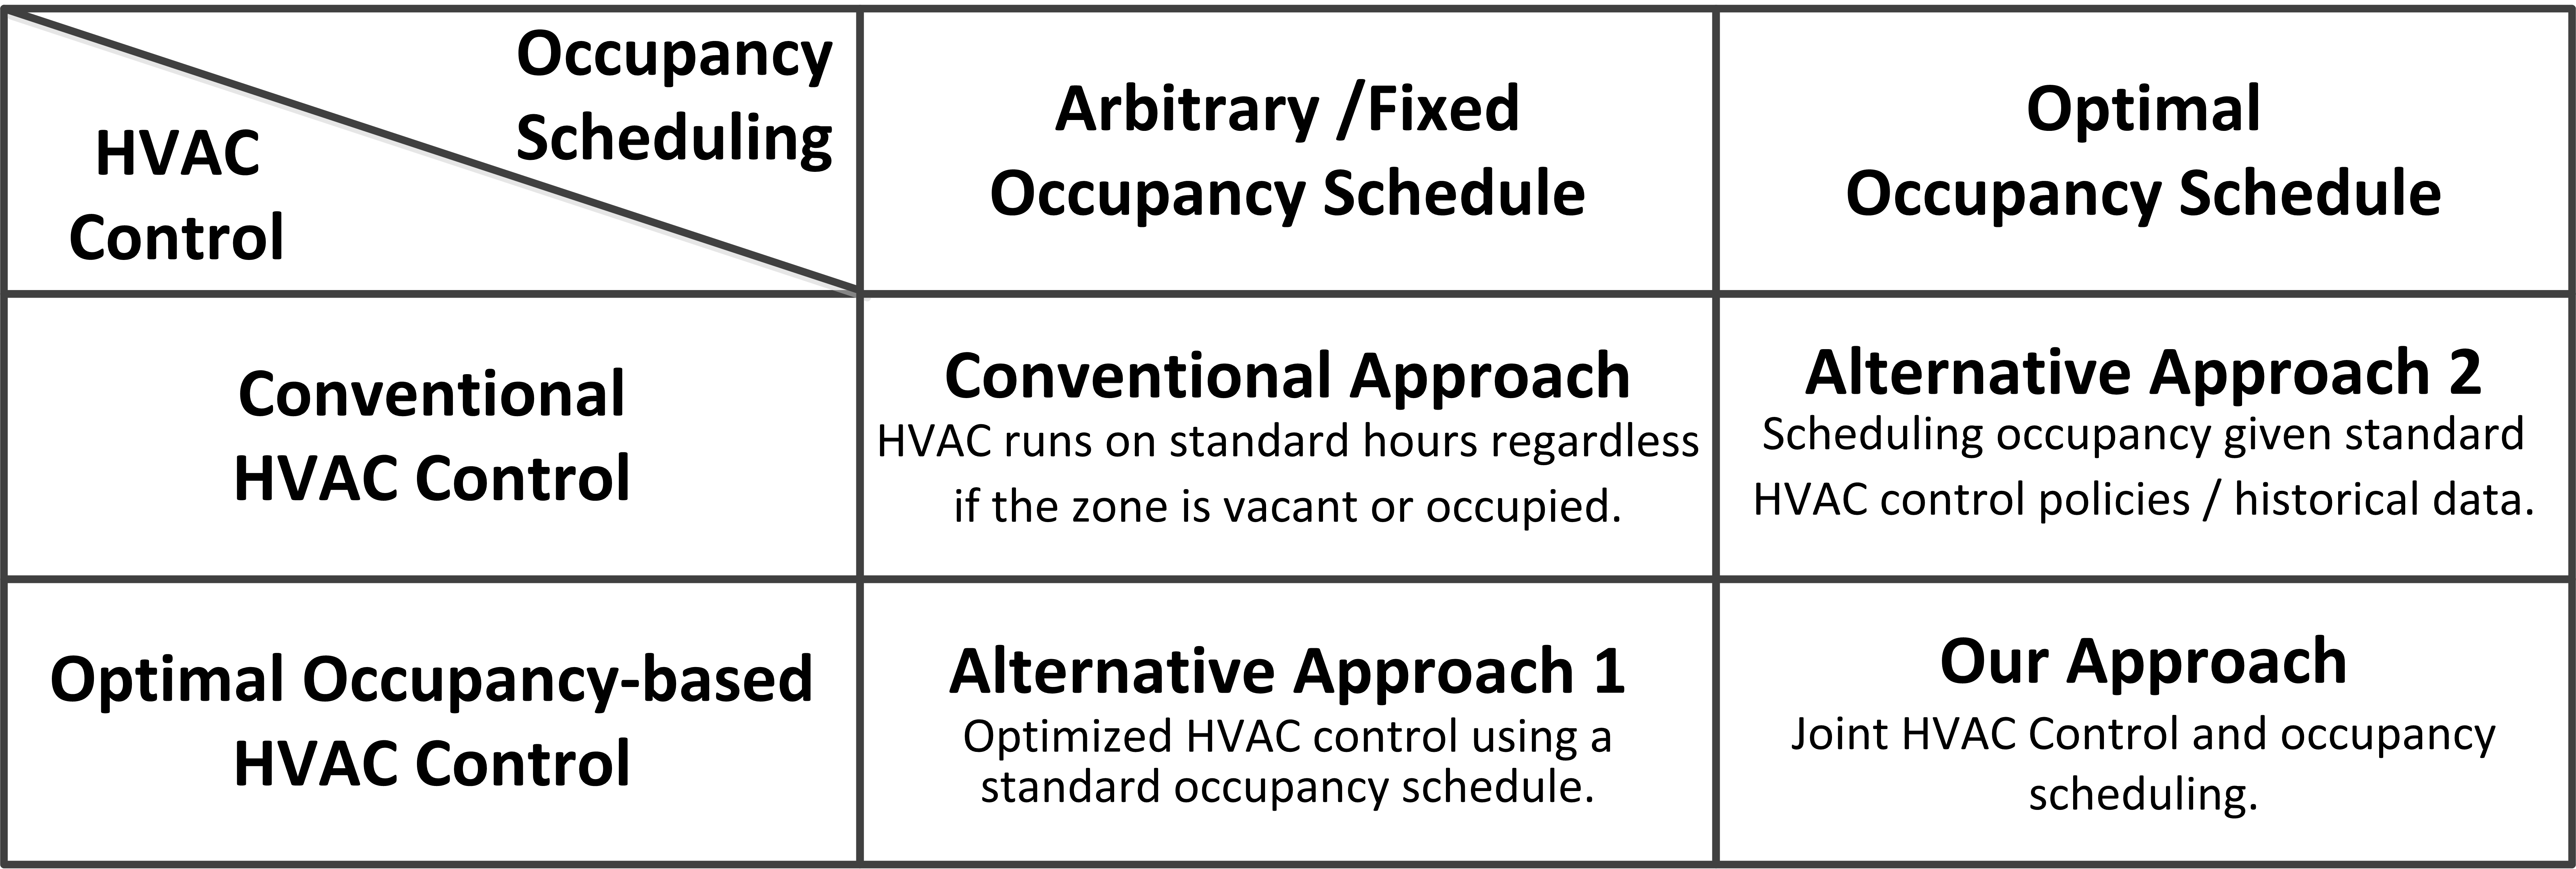
\includegraphics[width=0.74\linewidth,keepaspectratio]{./figs/mip_taxonomy.jpg}		
	\caption{HVAC control \& occupancy scheduling: existing approaches vs. our approach}
	\label{fig:mip_taxonomy}
\end{figure}

Energy consumption in commercial and educational buildings is impacted by group activities such as meetings, workshops, classes and exams.
%Group activities such as meetings, workshops, classes and exams impact the energy consumption in commercial and educational buildings.
Currently, most buildings adopt a conventional approach for managing HVAC systems. The building HVAC is turned on during business hours, typically 6am to 6pm, regardless whether a building zone is occupied or not. This widespread use of fixed schedule-based control constitutes to one of the main inefficiencies in building management system. We believe that energy consumption can be reduced by scheduling group activities to take place at times and locations that are favorable from an energy standpoint.

%As occupants influence the thermal behavior of buildings, 
Various optimisation approaches have been proposed to optimise HVAC utilisation using occupancy information. Figure \ref{fig:mip_taxonomy} shows a simple classification of the existing works on HVAC control and occupancy scheduling, and how our work differs from these state-of-the-art approaches. 

Moving away from the conventional approach, existing works consider only one of the solutions: 
\begin{itemize}
	\item Alternative Approach 1 (Optimal occupancy-based HVAC control-oriented) - The HVAC community focuses at optimising HVAC control using a standard occupancy schedule, or by ``detecting'' if a room is occupied based on sensors \citep{agarwal2010occupancy,goyal2013occupancy,brooks2015energy}. This approach does not perform any occupancy scheduling, and therefore it ignores the fact that there are better schedules that lead to higher energy savings.
	\item Alternative Approach 2 (Optimal occupancy scheduling-oriented) - The scheduling community focuses at optimising the occupancy schedule given standard HVAC control policies or historical data \citep{pan2012thermal,majumdar2012energy,kwak2013tesla,majumdar2016characterising}. They typically adopt suboptimal scheduling strategies guided by heuristics to search for solutions that take advantage of thermal inertia, and schedule activities by considering criteria include minimising the number of rooms used, minimising the time gap between activities in the same room, and minimising the gap between room capacity and the number of occupants.	An important limit of this line of research is that it adopts a black-box modeling approach to calculate HVAC energy consumption, and therefore it fails to exploit the advantage of occupancy HVAC control.
\end{itemize}


%You can do this and do that in sequence, but…. We can do more…. This is what we are doing…
%(after saying sequential step) ……  But (emphasize) we can do something better 

In this chapter, we show that combining HVAC control with occupancy scheduling can lead to substantial improvements in energy efficiency. 
We focus on improving the effectiveness of energy-aware room-booking and meeting scheduling approaches, by allowing the scheduling decisions to rely on an explicit model of the building's occupancy-based HVAC control. The core component of our approach is a mixed-integer linear programming (MILP) model which we use to optimally solve the joint occupancy scheduling and occupancy-based HVAC control problem. This joint problem consists in deciding the respective times and locations of a set of activities, as well as the HVAC supply air flow rate and air flow temperature for each zone and time, in such a way as to optimise the overall HVAC consumption over a receding horizon.

Our initial HVAC control model builds on well-accepted work by \cite{goyal2013occupancy}, but introduces a number of significant changes required to be suitable as a sub-component of our more complex joint scheduling and control model. Notably, the control model studied by \cite{goyal2013occupancy} is a purely continuous {\em non-linear} model which does not consider occupancy. Our experiments, which use the IPOPT solver \citep{Ipopt}, revealed that this model is impractical for our application, in terms of both memory and run-time requirements. In contrast, we formulate an efficient linear model that incorporates discrete variables to capture occupancy. % and after-hour standby mode.
The linear model is formulated by relaxing the non-linear HVAC control constraints in a principled way using McCormick Relaxation \citep{mccormick1976computability}. 

To enable joint optimisation between HVAC control and occupancy scheduling, we introduce a discrete variable that indicates if a location is being occupied by a scheduled activity, which then triggers a HVAC control constraint that ensures the room temperature is between the occupied thermal comfort bound. To ensure the existence of a feasible control for adequately sized HVACs and improve on the current occupancy-based HVAC control practices, we introduce a \textsl{standby mode} enabling the HVAC to re-activate at night if this is necessary to meet the temperature bounds of an early morning meeting or results in reduced consumption. Our experiments illustrate the circumstances under which the standby mode is beneficial, and show the superiority (over 50\% consumption reduction) of our joint MILP model compared to heuristic scheduling solutions and to more na\"{\i}ve integrations of meeting scheduling and occupancy-based HVAC control. 

In the following, we start by introducing the occupancy-based HVAC control aspects of our MILP model in Section \ref{sec:mip:control}. We describe in turn the type of HVAC system we focus on along with the objective function we consider, the bounds the control must comply with, the effect of the control on the building thermal dynamics, and the linear relaxation of the non-linear constraints. In Section \ref{sec:mip:scheduling} we will cover the scheduling aspects and demonstrate how the scheduling model can be integrated to the HVAC control. We provide experimental comparisons of our integrated model with the state-of-the-art in Section \ref{sec:mip:experiments}, followed by a discussion of the related work in Section \ref{sec:mip:related} and finally draw a conclusion in Section \ref{sec:mip:conclusion}. 

%To summarise, the main contributions of the paper are: a) an efficient MILP model for occupancy-based HVAC control which can be used in a range of applications, b) a scalable and effective approach to occupancy scheduling which exploits the capabilities of HVAC control and c) experiments showing a substantial reduction in energy consumption over the state of the art.

\section{Occupancy-Based HVAC Control}
\label{sec:mip:control}

%Following \citep{goyal2013occupancy}, 
We adopt a model predictive control (MPC) approach and consider variable-air-volume (VAV) based HVAC systems, which are widely
deployed in commercial buildings. With such systems, the building is divided into a number of zones (or locations) $L\subseteq\mathbb{N}$,
each of which can be an individual room or a group of rooms. Figure~\ref{fig:hvac} shows a schematic of a VAV system connected to two building zones.  To simplify notation, we assume that each zone corresponds to a
single room. %In the description of the model, values of constants are given between square brackets. 

\subsection{VAV System and Objective Function}
\begin{figure}
	\centering
		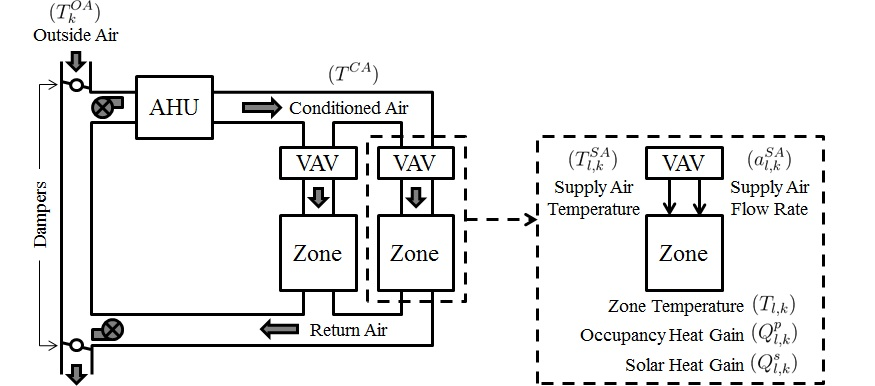
\includegraphics[width=0.74\linewidth,keepaspectratio]{./figs/vav_new.jpg}		
	\caption{VAV-based HVAC system with two zones}
	\label{fig:hvac}
\end{figure}

Let $K = \{1 \ldots n\}$ be a finite set of discrete time steps considered over the optimisation horizon. For simplicity, we assume
that successive time steps are separated by a fixed duration $\bm{\Delta t} \in \mathbb{R}^+$; that is, $\forall k\in K$, we have $t_k \in
\mathbb{R}^+$ and $t_{k} - t_{k-1} = \bm{\Delta t}$. The objective is to minimise the total energy consumed over the optimisation horizon:

\begin{equation} \label{eq:objective}
\mbox{minimise: } \sum_{k\in K} e_{k}
\end{equation}

\noindent where $e_k$ is the energy consumed at time step $k$: 
\begin{equation} \label{eq:e_total} 
e_{k} = p_{k} \times \bm{\Delta t} \hspace{20pt} \forall k \in K 
\end{equation}

\noindent The power $p_{k}$ is consumed by the three main operations shown in Figure~\ref{fig:hvac} and detailed below: the
  air conditioning operation performed centrally by the air handling unit (AHU) consumes $p_{k}^{Cond}$; the fan operation, also
  performed centrally, consumes $p_{k}^{Fan}$; and the reheating operation performed locally at each zone $l\in L$ by the zone's VAV
  unit consumes $p_{l,k}^{Heat}$:
	
\begin{equation} \label{eq:p_total} 
p_{k} = \left( p_{k}^{Cond} + p_{k}^{Fan} + \sum\limits_{l \in L} p_{l,k}^{Heat}\right) \hspace{10pt} \forall k \in K 
\end{equation}

We now provide the details of the power consumed by these 3 operations:

\noindent\emph{Air Conditioning Operation.} The AHU admits a mixture of outside air at temperature $\bm{T^{OA}}_k$ and
return air, and conditions it to a pre-set conditioned air temperature $\bm{T^{CA}}$ [usually $12.8\,^{\circ}\mathrm{C}$]. The conditioned air is then distributed through the supply duct to the VAV unit at each zone. The AHU consumption $p_{k}^{Cond}$ is the power consumed in cooling the total air flow required.  Let $a^{SA}_{l,k}$ denote the air flow rate required by location $l$ at time step $k$ and $\bm{C^{pa}}$ the heat capacity of air at constant pressure [1.005 kJ/kg$\cdot$K]: 

\begin{equation} \label{eq:p_cond}
p_{k}^{Cond} = \bm{C^{pa}}\left(\bm{T^{OA}_{k}} - \bm{T^{CA}}\right) \sum\limits_{l \in L} a_{l,k}^{SA} \hspace{10pt} \forall k \in K 
\end{equation}

\noindent\emph{Fan Operation.} The supply fan, driven by a variable frequency drive, maintains a constant static pressure in the supply
duct. When the opening of the VAV dampers increases to pull in more air flow into the conditioned space (resp. decreases to pull less air
flow), the fan speeds up (resp. slows down). The fan consumption is the power consumed to push the total air flow required through the
supply duct, which is proportional to the sum of the air flow rates $a^{SA}_{l,k}$ required over all locations. Let $\bm \beta$ be the fan
coefficient [0.65]: 

\begin{equation} \label{eq:p_fan}
p_{k}^{Fan} = \bm{\beta} \sum\limits_{l \in L} a_{l,k}^{SA} \hspace{20pt}  \forall k \in K
\end{equation}

\noindent\emph{Reheating Operation.} Each zone $l$ has a VAV unit connected to the supply duct. The unit is equipped with
continuously adjustable valves and reheat coils. These enable regulating the air flow rate $a^{SA}_{l,k}$ into the zone and
modulating the supply air temperature $T^{SA}_{l,k}$ to maintain the zone temperature within given bounds, if necessary by reheating the
supply air. Here we consider the power $p_{l,k}^{Heat}$ consumed by the reheating process to heat the supply air from the conditioned
temperature $\bm{T^{CA}}$ to an appropriate location supply air temperature $T_{l,k}^{SA}$.  

\begin{equation} \label{eq:p_heat} 
p_{l,k}^{Heat} = \bm{C^{pa}} (T_{l,k}^{SA}- \bm{T^{CA}}) a_{l,k}^{SA} \hspace{10pt} \forall l \in L,k \in K 
\end{equation}

\noindent\emph{Decision Variables.} The two key HVAC decision variables are the supply air flow rate $a_{l,k}^{SA}$ and
temperature $T_{l,k}^{SA}$ at each location $l \in L$ and time step $k\in K$. We determine an optimal control for these variables, given
occupancy information and bounds on supply air temperature, supply air flow rate, and room temperature during vacant and occupied
periods. Below we will introduce a third decision variable $w_{l,k}$ to decide when the HVAC should activate at night, which in turn will influence the bounds described below. When taking the HVAC control model in isolation, the building occupancy is an {\em input} to the model. When we integrate scheduling into the model in Section~\ref{sec:mip:scheduling}, occupancy will become a {\em decision variable}.

\subsection{Temperature and Air Flow Bounds}
We now model the constraints on the temperature, supply air temperature and supply air flow rate in each location, as a function
of the location occupancy and the time of the day.  We introduce the auxiliary variable $T_{l,k} \in \mathbb{R}$ representing the {\em
  actual} temperature in location $l\in L$ at time step $k\in K$, and the Boolean input $z_{l,k}$ which is true if and only if $l$ is occupied at time step $k$. When a location is not occupied, its temperature can lie freely within a wide temperature range $[\bm{\underline{T}^{\emptyset}}, \bm{\overline{T}^{\emptyset}}]$, whilst the temperature is otherwise constrained to lie within a more restricted comfort range $[\bm{\underline{T}^{\emptyset}} + \bm{\underline{T}^g}, \bm{\overline{T}^{\emptyset}}-\bm{\overline{T}^g}]$, where $\bm{\underline{T}^g}$ and $\bm{\overline{T}^g}$ are appropriate constants. This constraint is expressed as follows:

\begin{equation} \label{eq:temp_cstr}
\bm{\underline{T}^{\emptyset}} + \bm{\underline{T}^g} z_{l,k} \leq T_{l,k} \leq \bm{\overline{T}^{\emptyset}} - \bm{\overline{T}^g} z_{l,k} \quad \forall l\in L , k \in K 
\end{equation}

Further, the supply air temperature and flow rate at each location are constrained in a way that depends on the HVAC operating mode at the
current time step. We have two operating modes: {\em active} and {\em standby}. Let $K^{s} \subseteq K$ be the set of time steps that fall
within standard operating hours (6am to 6pm).  During standard hours ($k\in K^s$) the HVAC is always in active mode. The supply air
temperature $T^{SA}_{l,k}$ at location $l$ must fall within $[\bm{T^{CA}}, \oversl{\bm{T}}^{SA}]$. The supply air flow rate $a_{l,k}^{SA}$ must fall within $[\bm{\underline{a}^{SA}}_{l}, \bm{\overline{a}^{SA}}]$. The upper bound $\bm{\overline{a}^{SA}}$ [$5.0$ kg/s] is the air flow rate obtained when the dampers are fully open. The lower bound $\bm{\underline{a}^{SA}_l}$ is a constant calculated as a function of the area of the location, the factor of indoor air quality and the return air ratio necessary to ensure that the minimal fresh outside air requirements specified in the ASHRAE ventilation standard are met \citep{ashrae2013thermal}. 

\begin{equation} \label{eq:asalb}
% self.EAMS.ALPHA_IAQ_FACTOR_OF_SAFETY*((self.EAMS.MASS_AIR_FLOW_OUTSIDE_AIR_PER_METER_SQUARE * width * length * height) /
%                                                    (1-self.EAMS.MASS_AIR_FLOW_RETURN_AIR_RATIO))
\bm{\underline{a}_{l}^{SA}} = \bm{\alpha} \times \frac{\bm{a^{OA}} \times \bm{l^{width}} \times \bm{l^{length}}}{1-\bm{a^{RAR}}} \quad \forall l\in L
\end{equation}

\noindent In Equations \eqref{eq:asalb}, $\bm \alpha [1.7]$ is a constant coefficient that represent the indoor air quality safety factor. $\bm{a^{OA}}$ [0.36 g/s] denotes the minimum outside air flow rate required per square meter to ensure fresh air is being circulated into the room. $\bm{a^{RAR}}$ [0.4] defines the ratio of return air to mixed air flow rate. $\bm{l^{width}}$ and $\bm{l^{length}}$ are the room size. 

With these bounds, we have the following constraints:

%  0.36 g/s comes from 0.0255 Kg/s * (1-0.4) / (25m^2 * 1.7) * 1000

\begin{equation} \label{eq:hvac_active_TSA}
\bm{T^{CA}} \leq T_{l,k}^{SA} \leq \bm{\overline{T}^{SA}}  \quad \forall l \in L, k\in K^s
\end{equation}

\begin{equation} \label{eq:hvac_active_ASA}
\bm{\underline{a}^{SA}}_{l} \leq a_{l,k}^{SA}  \leq \bm{\overline{a}^{SA}}   \quad \forall l \in L, k\in K^s
\end{equation}

Outside business hours ($k\in K\setminus K^s$), the HVAC is in stand-by mode and will only activate if this enables or lowers the
cost of satisfying a future constraint. For instance, it could activate at night and benefit from the low outside night temperature
to more cheaply cool the supply air to meet the temperature bounds in Constraints \eqref{eq:temp_cstr} for an early morning meeting. Note that this is different from conventional operations where HVACs are always off at outside hours; as our experiments will show, the standby mode enables model-predictive approaches to occupancy-based control to meet constraints and save energy. The decision of whether or not HVAC
activation is required by location $l$ is represented by the boolean decision variable $w_{l,k}$. The presence of these boolean variables
makes our model a mixed-integer model. When $w_{l,k}$ is true, the supply air temperature and air flow rate are constrained to lie within
$[\bm{T^{CA}}, \bm{\overline{T}^{SA}}]$ and $[\bm{\underline{a}^{SA}}_{l},\bm{\overline{a}^{SA}}]$, respectively, and when $w_{l,k}$ is false, $a_{l,k}^{SA}$ is set to zero and the value of $T_{l,k}^{SA}$ is irrelevant (and for simplicity may as well also be zero). This is captured by the following
constraints:

\begin{equation} \label{eq:hvac_standby_TSA}
\bm{T^{CA}} w_{l,k} \leq T_{l,k}^{SA} \leq \bm{\overline{T}^{SA}} w_{l,k}  \quad \forall l \in L, k \in K \setminus K^s
\end{equation}

\begin{equation} \label{eq:hvac_standby_ASA}
\bm{\underline{a}^{SA}}_{l} w_{l,k} \leq a_{l,k}^{SA} \leq \bm{\overline{a}^{SA}} w_{l,k}  \quad \forall l \in L, k \in K \setminus K^s
\end{equation}

\subsection{Building Thermal Dynamics} \label{mip:thermal}
Having defined the space of decisions as the supply air flow rate $a_{l,k}^{SA}$, the supply air temperature $T_{l,k}^{SA}$ and the HVAC
activation requirement $w_{l,k}$ at each location and time step, we now model the impact of these decisions on the building thermal
exchanges.  To model the thermal dynamics of the building, we adopt a computationally efficient lumped RC-network \citep{gouda2000low} which
incorporates the thermal resistance and capacitance of each zone and between adjacent zones, as well as the solar gain and the internal
heat gain in each zone -- in particular the heat gain arising from occupancy. For the sake of simplicity, we ignore humidity and
infiltration.

\begin{figure}[t]
\centering
	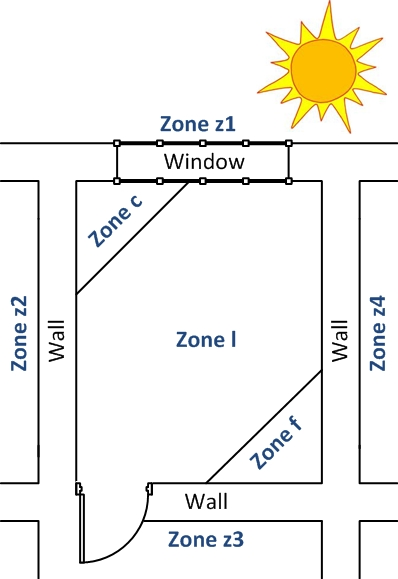
\includegraphics[width=2.5in,keepaspectratio]{./figs/zone1.jpg}
\caption{Zone}
\label{fig:zone}
\end{figure}

\begin{figure}[t]
\centering
	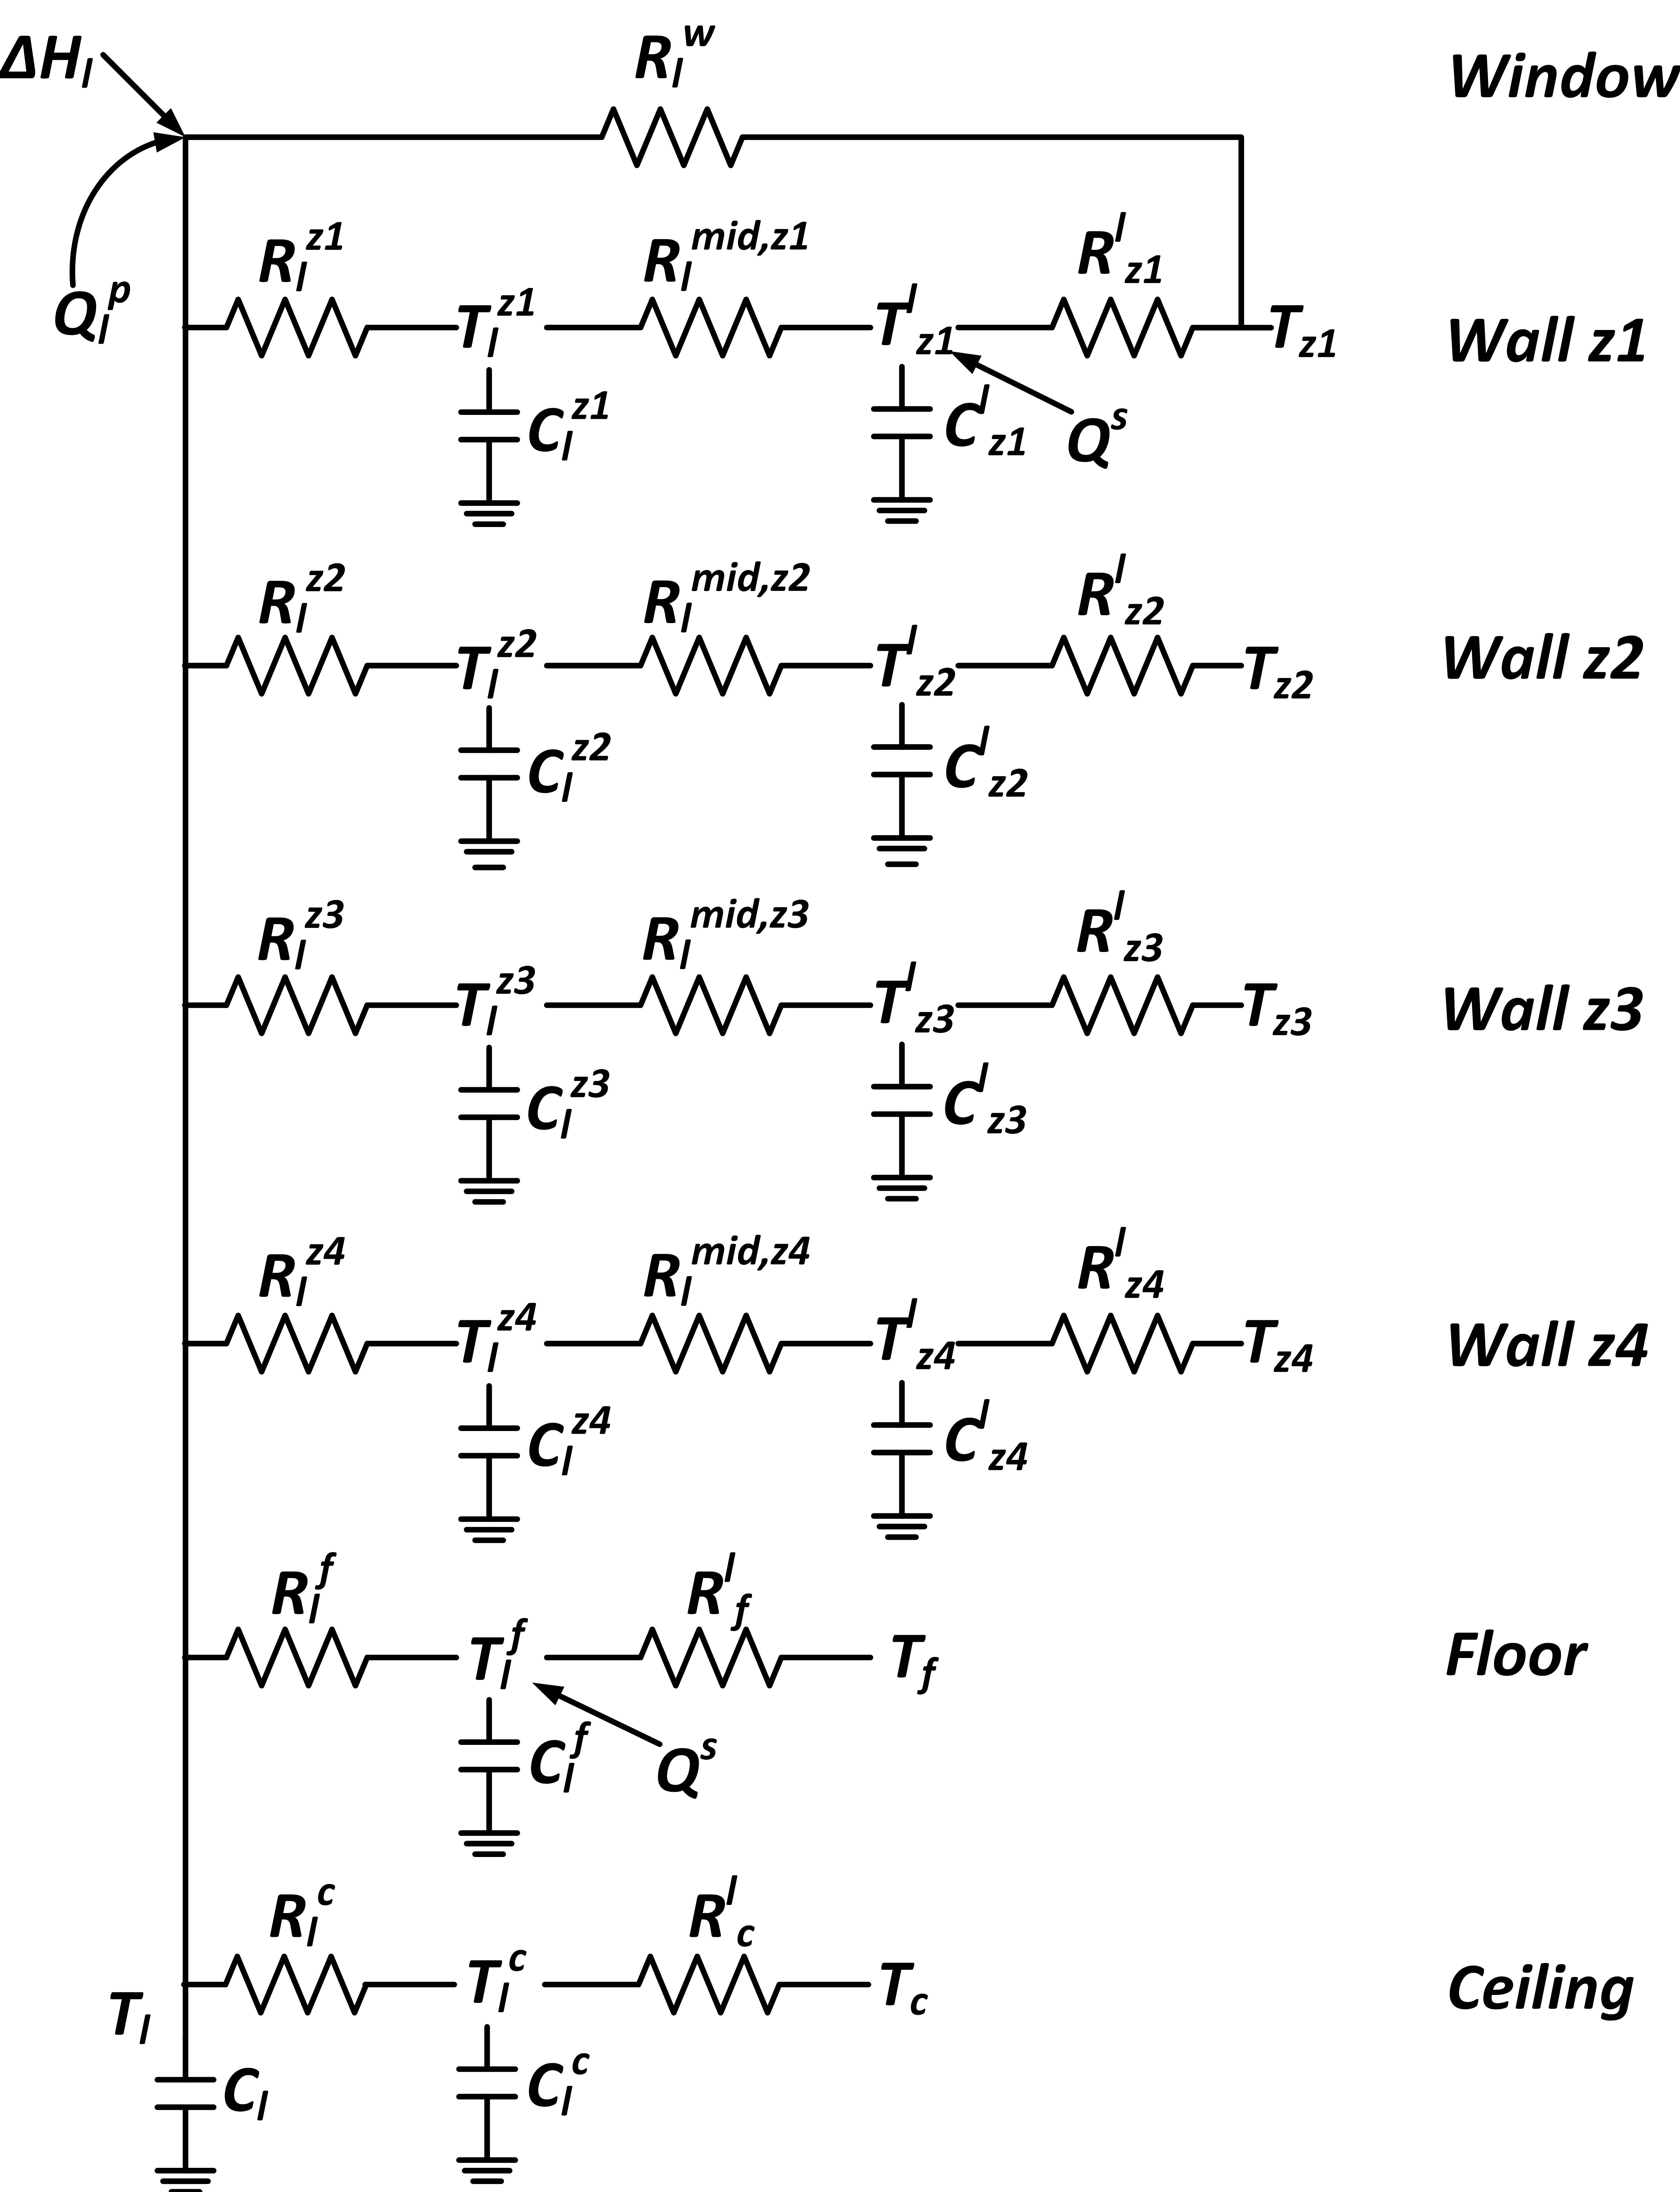
\includegraphics[width=4.0in,keepaspectratio]{./figs/3r2c.jpg}
\caption{Lumped-RC Network}
\label{fig:network}
\end{figure}

The principles behind the thermal model are represented in Figure \ref{fig:zone} and Figure \ref{fig:network}. Figure \ref{fig:zone} shows the zone structure that we adopt. Zone $l$ is separated by a wall and a window from zone $z1$ and by a wall from zones $z2$, $z3$, and $z4$, which could represent either indoor or outdoor zones. It is also separated by the ceiling and floor from zones $c$ and $f$ which are above and below zone $l$, respectively. Zone $l$ has a capacitance $\bm{C_l}$ that models the heat capacity of the air in the zone.  It also has a solar gain $Q^{s}_{l,k}$ and heat gain $Q^{p}_{l,k}$ at time step $k$. Moreover, the inner (resp. outer) wall separating $l$ from zone $z\in Z= \left\{z1,z2,z3,z4,f,c\right\}$ has a capacitance $\bm{C^z_l}$ (resp. $\bm{C^l_z}$), resistance $\bm{R^z_l}$ (resp. $\bm{R^l_z}$), and temperature $T^z_{l,k}$ (resp. $T^l_{z,k}$) at time step $k$. The window has a resistance $\bm{R^w_l}$. Finally, the internal node between the inner and outer walls separating $l$ from $z\in\{z1,z2,z3,z4\}$ has a constant resistance $\bm{R^{mid,z}_l}$. Capacitances, resistances, solar gain, and (in this section) occupant heat gain are inputs to the model whilst temperatures are auxiliary variables. The interaction between zones is modeled using a lumped RC-network. Specifically, we use 3R2C for walls separating two zones, 2R1C for the ceiling and floor and 1R for windows. The lumped network for Figure~\ref{fig:zone} is given in Figure~\ref{fig:network}.

The lumped network translates into a set of coupled difference equations which can be summarised as follows. The first difference equation defines the temperature $T_{l,k}$ in zone $l$ at time step $k$ as a function of the location, inner walls, ceiling, floor and outdoor temperatures at the previous time step, of the heat gain $Q^p_{l,k-1}$ at the previous time step and of the enthalpy $\Delta H_{l,k-1}$ of the location due to the supply air: 

\begin{equation}\label{eq:roomtemperature}
\begin{split}
{T}_{l,k} = 
\left[ 1 - \frac{\bm{\Delta t}}{\bm{C_l}} (\sum_{z\in Z} \frac{1}{\bm{R^z_l}} + \frac{1}{\bm{R^w_l}})  \right] T_{l,k-1} + 
\sum_{z\in Z} \frac{\bm{\Delta t}}{{\bm{C_l}}{\bm{R^z_l}}} T^{z}_{l,k-1} + 
\frac{\bm{\Delta t}}{{\bm{C_l}}\bm{{R^{w}_l}}} \bm{T^{OA}_{k-1}} 
& + \frac{\bm{\Delta t}}{\bm{C_l}} \Delta H_{l,k-1} \\
& + \frac{\bm{\Delta t}}{\bm{C_l}} Q^{p}_{l,k-1} 
\end{split}
\end{equation}

%
%\begin{equation} \label{eq:roomtemperature}
%\begin{split}
%\frac{{C}_l}{\Delta t}({T}_{l,k} -T_{l,k-1}) = 
%- \left[
%\sum_{z\in Z} \frac{1}{\bm{R^z_l}} +
%\frac{1}{\bm{R^w_l}}
%\right] T_{l,k-1} \\
%+ \sum_{z\in Z}\frac{T^{z}_{l,k-1}}{\bm{R^z_l}} +
%\frac{\bm{T^{OA}_{k-1}}}{\bm{R^w_l}}
%+ Q^{p}_{l,k-1} + \Delta H_{l,k-1}
%\end{split}
%\end{equation}

\noindent The heat gain $Q^p_{l,k}$ is simply the heat gain $q^p$ generated per person (75W), times the number of occupants $pp_{l,k}$:
\begin{equation} \label{eq:heatgain}
Q^{p}_{l,k} = \bm{q^{p}} \times pp_{l,k}
\end{equation}

\noindent Ignoring humidity, the enthalpy is defined as follows:
\begin{equation} \label{eq:enthalpy}
\Delta H_{l,k} = \bm{C^{pa}} a^{SA}_{l,k} (T^{SA}_{l,k} - T_{l,k})
\end{equation}
%\vspace*{-1px}
The remaining difference equations define the temperatures $T^z_{l,k}$ and $T^l_{z,k}$ of the inner and outer walls at time step $k$ as a
function of each other and of the location temperature $T_{l,k-1}$ at the previous time step. 

Taking $z=z1$ in the example of Figure~\ref{fig:zone}:

\begin{equation}\label{eq:temp:outer}
T^{z}_{l,k} = 
\left[ 1 - \frac{\bm{\Delta t}}{\bm{C_l^z}} (\frac{1}{\bm{R^z_l}} +  \frac{1}{\bm{R^{mid,z}_l}} )  \right] T^{z}_{l,k-1} + 
\frac{\bm{\Delta t}}{{\bm{C_l^z}}{\bm{R^z_l}}} T_{l,k-1} + 
\frac{\bm{\Delta t}}{{\bm{C_l^z}}{\bm{R^{mid,z}_l}}} T^{l}_{z,k-1} 
\end{equation}

\begin{equation}\label{eq:temp:inner}
T^{l}_{z,k} = 
\left[ 1 - \frac{\bm{\Delta t}}{\bm{C_z^l}} (\frac{1}{{R}^{l}_z} +  \frac{1}{\bm{R^{mid,z}_l}} )  \right] T^{l}_{z,k-1} + 
\frac{\bm{\Delta t}}{{\bm{C_z^l}}{\bm{R^l_z}}} \bm{T^{OA}_{k-1}} + 
\frac{\bm{\Delta t}}{{\bm{C_z^l}}{\bm{R^{mid,z}_l}}} T^{z}_{l,k-1} +
\frac{\bm{\Delta t}}{{\bm{C_z^l}}} \bm{Q^{s}_{l,k-1}}
\end{equation}

\noindent Observe that the definition of the inner wall temperature $T^{z}_{l,k}$ is symmetrical to that of the outer wall temperature $T^{l}_{z,k}$ except for the absence of solar gain $\bm{Q^s_{k-1}}$, and the replacement of the outdoor temperature $\bm{T^{OA}_{k-1}}$ with the room temperature $T^{z}_{l,k-1}$ of the neighbouring zone $z$.

%Note that if location $l$ has a wall separating it from room $z$, then $\bm{T^{OA}_{k-1}}$ is replaced by $T^{z}_{l,k-1}$
%Note that if location $l$ has a wall that separate between two rooms instead of the outdoor environment, $\frac{\Delta t}{{\bm{C_z^l}}{\bm{R^l_z}}} \bm{T^{OA}_{k-1}}$ is replaced with $\frac{\Delta t}{{\bm{C_z^l}}{\bm{R^l_z}}} T_{nl, k-1}$ where $nl$ is the neighbouring zone $l$. The equations for the other walls are similar, so we omit them here.

The temperatures of the floor and the ceiling at time step $k$ is calculated as a function of the location temperature $T_{l,k-1}$, the outdoor temperature $\bm{T^{OA}}$ and the solar gain $Q^{s}$ at the previous time step. 
\begin{equation}\label{eq:tlf}
T^{f}_{l,k} = 
\left[ 1 - \frac{\bm{\Delta t}}{\bm{C_l^f}} (\frac{1}{\bm{R^f_l}} +  \frac{1}{\bm{R^l_f}} )  \right] T^{f}_{l,k-1} + 
\frac{\bm{\Delta t}}{{\bm{C_l^f}}{\bm{R^f_l}}} T_{l,k-1} + 
\frac{\bm{\Delta t}}{{\bm{C_l^f}}{\bm{R^l_f}}} \bm{T^{OA}_{k-1}} +
\frac{\bm{\Delta t}}{{\bm{C_l^f}}} \bm{Q^{s}_{l,k-1}}
\end{equation}

\begin{equation}\label{eq:tlc}
T^{c}_{l,k} = 
\left[ 1 - \frac{\bm{\Delta t}}{\bm{C_l^c}} (\frac{1}{\bm{R^c_l}} +  \frac{1}{\bm{R^l_c}} )  \right] T^{c}_{l,k-1} + 
\frac{\bm{\Delta t}}{{\bm{C_l^c}}{\bm{R^c_l}}} T_{l,k-1} + 
\frac{\bm{\Delta t}}{{\bm{C_l^c}}{\bm{R^l_c}}} \bm{T^{OA}_{k-1}} 
\end{equation}

%\begin{equation} \label{eq:temp:outer}
	%\begin{split}
	%\frac{{C}^{l}_{z1}}{\Delta t} (T^{l}_{z1,k} \!-\! T^{l}_{z1,k-1}) =
		%- \left[
		%\frac{1}{{R}^{l}_{z1}} +
		%\frac{1}{{R}^{mid,z1}_l}
				%\right] T^{l}_{z1,k-1} 
		%+\frac{T_{z1,k-1}}{{R}^{l}_{z1}} +
                  %\frac{T^{z1}_{l,k-1}}{{R}^{mid,z1}_l} +
		%Q^s_{k-1}
	%\end{split}
%\end{equation}


\subsection{MILP Relaxation}
\label{subsec:relaxation}
Observe that the model as presented so far is a mixed-integer {\em non-linear} (MINLP) model. This is because of the bilinear terms $a_{l,k}^{SA}T_{l,k}^{SA}$ and $a_{l,k}^{SA}T_{l,k}$ in Equations~\eqref{eq:p_heat} and~\eqref{eq:enthalpy}. From a computational standpoint, it is better to relax these equations so as to obtain a MILP for which effective solvers exist that are guaranteed to return a lower bound on the globally optimal MINLP objective.  To obtain a suitable MILP, we use the linear programming relaxation of bilinear terms introduced by \cite{mccormick1976computability}. This relaxation introduces a new variable $v$ for the bilinear term $xy$ together with four
inequalities that define its convex envelope using the bounds $[\underline{x},\overline{x}]$ and $[\underline{y},\overline{y}]$ on each of the two variables involved:

\[\begin{array}{l}
v \geq \underline{x}y + \underline{y}x - \underline{x}\underline{y}\\
v \geq \overline{x}y + \overline{y}x - \overline{x}\overline{y}\\
v \leq \underline{x}y + \overline{y}x - \underline{x}\overline{y}\\
v \leq \overline{x}y + \underline{y}x - \overline{x}\underline{y}
\end{array}
\]

Hence, our MILP model is obtained by replacing the bilinear terms $a_{l,k}^{SA}T_{l,k}^{SA}$ with new variable $aT_{l,k}^{SA,SA}$ and $a_{l,k}^{SA}T_{l,k}$ with new variable $aT_{l,k}^{SA,z}$ in Equations~\eqref{eq:p_heat} and~\eqref{eq:enthalpy} and adding the corresponding convex envelope definitions. 

The new variable $aT_{l,k}^{SA,SA}$ is constrained by:
\begin{equation}
aT_{l,k}^{SA,SA} \geq \bm{\underline{a}^{SA}_{l,k}} T_{l,k}^{SA} + \bm{\underline{T}^{SA}_{l,k}} a_{l,k}^{SA} - \bm{\underline{a}^{SA}_{l,k}} \bm{\underline{T}^{SA}_{l,k}}\hspace{10pt} \forall l \in L, k \in K 
\end{equation}
\begin{equation}
aT_{l,k}^{SA,SA} \geq \bm{\overline{a}^{SA}_{l,k}} T_{l,k}^{SA} + \bm{\overline{T}^{SA}_{l,k}} a_{l,k}^{SA} - \bm{\overline{a}^{SA}_{l,k}} \bm{\overline{T}^{SA}_{l,k}}\hspace{10pt} \forall l \in L, k \in K 
\end{equation}
\begin{equation}
aT_{l,k}^{SA,SA} \leq  \bm{\underline{a}^{SA}_{l,k}} T_{l,k}^{SA} + \bm{\overline{T}^{SA}_{l,k}} a_{l,k}^{SA} - \bm{\underline{a}^{SA}_{l,k}} \bm{\overline{T}^{SA}_{l,k}}\hspace{10pt} \forall l \in L, k \in K 
\end{equation}
\begin{equation}
aT_{l,k}^{SA,SA} \leq  \bm{\overline{a}^{SA}_{l,k}} T_{l,k}^{SA} + \bm{\underline{T}^{SA}_{l,k}} a_{l,k}^{SA} - \bm{\overline{a}^{SA}_{l,k}} \bm{\underline{T}^{SA}_{l,k}}\hspace{10pt} \forall l \in L, k \in K 
\end{equation}

The new variable $aT_{l,k}^{SA,z}$ is constrained by:
\begin{equation} \label{eq:aSAT1} 
aT_{l,k}^{SA,z} \geq \bm{\underline{a}^{SA}_{l,k}} T_{l,k} + \bm{\underline{T}_{l,k}} a_{l,k}^{SA} - \bm{\underline{a}^{SA}_{l,k}} \bm{\underline{T}_{l,k}}  \hspace{10pt} \forall l \in L, k \in K 
\end{equation}
\begin{equation} \label{eq:aSAT2} 
aT_{l,k}^{SA,z} \geq \bm{\overline{a}^{SA}_{l,k}} T_{l,k} + \bm{\overline{T}_{l,k}} a_{l,k}^{SA} - \bm{\overline{a}^{SA}_{l,k}} \bm{\overline{T}_{l,k}} \hspace{10pt} \forall l \in L, k \in K 
\end{equation}
\begin{equation} \label{eq:aSAT3} 
aT_{l,k}^{SA,z} \leq  \bm{\underline{a}^{SA}_{l,k}} T_{l,k} + \bm{\overline{T}_{l,k}} a_{l,k}^{SA} - \bm{\underline{a}^{SA}_{l,k}} \bm{\overline{T}_{l,k}} \hspace{10pt} \forall l \in L, k \in K 
\end{equation}
\begin{equation} \label{eq:aSAT4} 
aT_{l,k}^{SA,z} \leq  \bm{\overline{a}^{SA}_{l,k}} T_{l,k} + \bm{\underline{T}_{l,k}} a_{l,k}^{SA} - \bm{\overline{a}^{SA}_{l,k}} \bm{\underline{T}_{l,k}}  \hspace{10pt} \forall l \in L, k \in K 
\end{equation}

The relevant bounds are:

\begin{itemize}
\item $a_{l,k}^{SA} \in [\bm{\underline{a}^{SA}_{l,k}}, \bm{\overline{a}^{SA}_{l,k}}] = 
\left\{
\begin{array}{ll}
\![\bm{\underline{a}^{SA}},\bm{\overline{a}^{SA}}_l] & \mbox{for $k\in K^s$}\\
\![0,\bm{\overline{a}^{SA}}] & \mbox{for $k\in K\setminus K^s$}\\
\end{array}
\right.$

\item $T_{l,k}^{SA} \in [\bm{\underline{T}^{SA}_{l,k}}, \bm{\overline{T}^{SA}_{l,k}}] = 
\left\{
\begin{array}{ll}
\![\bm{T^{CA}},\bm{\overline{T}^{SA}}] & \mbox{for $k \in K^s$}\\
\![0,\bm{\overline{T}^{SA}}] & \mbox{for $k \in K \setminus K^s$}\\
\end{array}
\right.$

\item $T_{l,k}\in [\underline{T}_{l,k}, \overline{T}_{l,k}] = [\undersl{\bm T}^{\bm \emptyset} ,\oversl{\bm T}^{\bm \emptyset} ]$ for $k\in K$
\end{itemize}

This concludes the description of our MILP model for occupancy-based HVAC control. Given the occupancy $pp_{l,k}$ and $z_{l,k}$, and the
external temperature $\bm{T^{OA}_{k}}$, it controls the supply air flow rate $a^{SA}_{l,k}$ and temperature $T^{SA}_{l,k}$ and decides when a
location requires HVAC activation $w_{l,k}$ out of the standby mode, in such a way as to optimise the total energy consumption $\sum_{k\in
  K}e_k$. The strengths of this model are its integration of realism and computational efficiency, its adequacy as a component of occupancy
scheduling and other more complex models, and its optional ability to activate out of the standby mode when this improves consumption.

\vspace*{10ex}
\section{Occupancy Scheduling}
\label{sec:mip:scheduling}
%\vspace*{-1ex}
Until now, zone occupancy over time was a model input. We now present our joint HVAC control and meeting scheduling model, in which occupancy is a decision variable.

Let $M \subseteq \mathbb{N}$ be a set of meetings to be scheduled to take place at the locations in $L$ during the time horizon $K$. Each meeting $m\in M$ is characterised by the following inputs: its duration $d_{m} \in \mathbb{N}$ (number of time steps), the set of allowable time steps $K_m \subseteq K$ at which it can start, the set of allowable locations $L_m\subseteq M$ at which it can take place, and its set of attendees $P_m \subseteq A$, for some appropriate set of attendees $A$. In addition, let ${\cal C}(M) \subseteq 2^{M}$ be the set of meeting sets which have at least one attendee in common, that is ${\cal C}(M)=\{C\subseteq M \mid \forall m,m'\in C, P_m\cap P_{m'} \neq \emptyset \}$.  In practice, only pairs of incompatible meetings are needed. Note that the sets $K_m$ and $L_m$ can be used to encode a variety of situations, such as room capacity requirements and availability of special equipment such as video conferencing, as well as time deadlines for the meeting occurrence and attendee availability constraints.

The main scheduling variable is the boolean decision variable $x_{m,l,k}$ which is true if meeting $m\in M$ is scheduled to take place at location $l\in L_m$ starting at time step $k\in K_m$. The scheduling part of the model interacts with the HVAC control part via the auxiliary variables $z_{l,k}$, which, as before, is true if location $l$ is occupied at time step $k$, and $pp_{l,k} \in \mathbb{N}$, which, as before, represents the number of occupants at location $l$ at time step $k$. These terms are used in Equations~\eqref{eq:temp_cstr} and~\eqref{eq:heatgain}, respectively, but are now variables rather than inputs.

The set of MILP scheduling constraints are the following. The first constraints ensure that all meetings are scheduled to occur exactly once within the range of allowable locations and start times: 
\begin{equation} \label{eq:ms_every} 
\mathop{\sum \limits_{l\in L_m, k \in K_m}} x_{m,l,k}=1 \hspace{10pt} \forall m \in M 
\end{equation}

\noindent The second constraints ensure that if a location is occupied by a meeting then it is exclusively occupied by this meeting during
its entire duration: 
\begin{equation} \label{eq:ms_totalalloc} 
\mathop{\sum \limits_{\substack{m \in M, k' \in K_m\\ {\scriptsize \mbox{~such that~}}\\ l\in L_m {\scriptsize \mbox{~and~}} k-d_m+1 \leq k' \leq k}}} x_{m,l,k'} \leq z_{l,k} \hspace{10pt} \forall l \in L, k \in K
\end{equation}
						
\noindent As a result, no two meetings can occupy the same location at the same time step. Observe that Constraints \eqref{eq:ms_totalalloc} also determine the occupancy variable $z_{l,k}$ used in the occupancy-based HVAC control part of the joint model.

The following constraints establish the number of occupants $pp_{l,k}$ of each location $l$ at each time step $k$:
\begin{equation} \label{eq:ms_totalnum} 
\mathop{\sum \limits_{\substack{m
        \in M, k' \in K_m\\ {\scriptsize \mbox{~such that~}}\\ l\in
        L_m {\scriptsize \mbox{~and~}} k-d_m+1 \leq k' \leq
        k}}} x_{m,l,k'}\times \left| P_m\right| =
  {pp}_{l,k} \hspace{8pt} \forall l \in L, k \in K 
\end{equation}

\noindent This is used in Equations~\eqref{eq:heatgain} to establish the internal heat gain arising from occupancy.

Finally, the last constraints ensure that meetings with an intersecting attendee set cannot overlap in time:
\begin{equation} \label{eq:ms_meeting}
\mathop{\sum \limits_{\substack{m \in \nu, l \in L_m, k' \in K_m\\ 
{\scriptsize \mbox{~such that~}}\\
k-d_m+1 \leq k' \leq k}}}  x_{m,l,k'} \leq 1 \hspace{10pt} \forall k \in K, \nu \in {\cal C}(M)
\end{equation}

Our joint HVAC control and occupancy scheduling model is simply obtained by adding Equations~\eqref{eq:ms_every}-\eqref{eq:ms_meeting} to the HVAC control model given by Equations~\eqref{eq:objective}-\eqref{eq:aSAT4}. Equations~\eqref{eq:p_heat} and Equations~\eqref{eq:enthalpy} are linearised by replacing the bilinear term $a^{SA}_{l,k}T^{SA}_{l,k}$ with $aT^{SA,SA}_{l,k}$ and $a^{SA}_{l,k}T_{l,k}$ with $aT^{SA,z}_{l,k}$.  The model optimises the total energy consumed not only over the HVAC decision variables $a^{SA}_{l,k}$, $T^{SA}_{l,k}$ and $w_{l,k}$ as before, but also over the scheduling decision variables $x_{m,l,k}$. A building occupancy-based HVAC controller need only use the schedules $x_{m,l,k}$ produced. A conventional controller may instead use the bounds on room temperature and supply air flow rate/temperature determined by Equations~\eqref{eq:temp_cstr}, \eqref{eq:hvac_active_TSA} and~\eqref{eq:hvac_standby_ASA} as setpoints. 

This concludes the description of our joint HVAC control and occupancy scheduling model. The next section experimentally investigates its
benefits in terms of energy reduction, in comparison with more na\"{\i}ve integrations of scheduling and HVAC control. 


\section{Experiments}
\label{sec:mip:experiments}

Our experiments aim at assessing the impact of room and time slot selections to HVAC consumption, explaining the usefulness of the standby mode and demonstrating that our HVAC-aware scheduling model leads to significant consumption reduction (50\% to 70\% in our experiments) when compared to occupancy-based HVAC control using arbitrary schedules or energy-aware schedules generated by heuristic methods. 

Simulations are carried out for five different building types with similar geometry but with different thermal resistance and capacitance. They are referred to as building type 1--5 in Table \ref{tab:rc_wall_win}. Each building corresponds to a row of 4 co-located zones (or interchangeably, rooms), where all zones have the same geometric area of $6\times 10\times 3 \mbox{ m}^3$ with a window surface area of $4\times 2    \mbox{ m}^2$. The two middle zones have two external walls (the wall separates the zone to the outside), with an area size of $6\times 3 \mbox{ m}^2$ each. The corner zones have an additional $3\times 10 \mbox{ m}^2$ of external wall. All the other walls of the zone are called internal walls. Two adjacent zones are separated with an internal wall. The thermal capacitance and thermal resistance for each wall at each building types are empirically designed based on construction materials obtained from \cite{gouda2000low}, \cite{gouda2002building}, \cite{goyal2013occupancy} and \cite{ashrae2013fund}. The outdoor temperature is taken from the month of January in Canberra, Australia, which is a summer month in the Southern hemisphere. The solar gain ranges from 50 to 350 W/m$^2$ during the day. Each room has a capacity of 30 people. The duration between successive time steps is $\bm{\Delta t} = 30$min, giving more than enough time for thermal effects to occur.  The MILP models are solved using Gurobi 5.6 \citep{gurobi}. All experiments were conducted on a cluster consisting of $2\times$ AMD 6-Core Opteron 4184, 2.8 GHz with 64 GB of memory.

\begin{table*}[t]
\centering
\begin{tabular}{p{0.2\linewidth} p{0.1\linewidth} p{0.1\linewidth}  p{0.1\linewidth} p{0.1\linewidth} p{0.1\linewidth}}
\hline\centering{Building Types} & \multicolumn{2}{c}{External Wall} & \multicolumn{2}{c}{Internal Wall} & {Window} \tabularnewline
       & \centering{(TR)} & \centering{(TC)} & \centering{(TR)} & \centering{(TC)} & \centering{(TR)} \tabularnewline
\hline \centering{1 (LRLC)} & \centering{3} & \centering{120} & \centering{1.5} & \centering{120} & \centering{0.5} \tabularnewline
\hline \centering{2 (MRMC)} & \centering{3} & \centering{140} & \centering{1.5} & \centering{140} & \centering{0.5} \tabularnewline
\hline \centering{3 (LRHC)} & \centering{3} & \centering{240} & \centering{1.5} & \centering{240} & \centering{0.5} \tabularnewline
\hline \centering{4 (HRLC)} & \centering{6} & \centering{120} & \centering{3} & \centering{120} & \centering{0.5} \tabularnewline
\hline \centering{5 (HRHC)} & \centering{6} & \centering{240} & \centering{3} & \centering{240} & \centering{0.5} \tabularnewline
\end{tabular}
	\caption{Total thermal resistance (TR) $\left( m^2 K\over W\right)$ and thermal capacitance (TC) $\left( KJ \over m^2K \right)$ of the walls and the window for five types of zones. The zones differ by a high (H), medium (M) and low (L) value for their thermal resistance (R) and capacitance (C). R and C of each wall can be derived by dividing TR and multiplying TC with area size respectively.}
	\label{tab:rc_wall_win}
\end{table*}


\subsection{Impacts of Room Selections and Time Allocations}

We start by studying the impact of room selections and time allocations for meetings on the HVAC consumption, through three simple case studies. We strive to answer two questions:
\begin{enumerate}
	\item Does room selection impact HVAC consumption?
	\item Does time allocation impact HVAC consumption?
	%\item Does room selection and time allocation impact HVAC control?
\end{enumerate}
\noindent Our goal is to provide evidence that room and time selections are crucial to reduce HVAC consumption.

\vspace{10px}
\emph{Case Study 1} \quad \textsl{How do building materials impact room temperature?}
\vspace{10px}

\begin{figure}
	\centering
		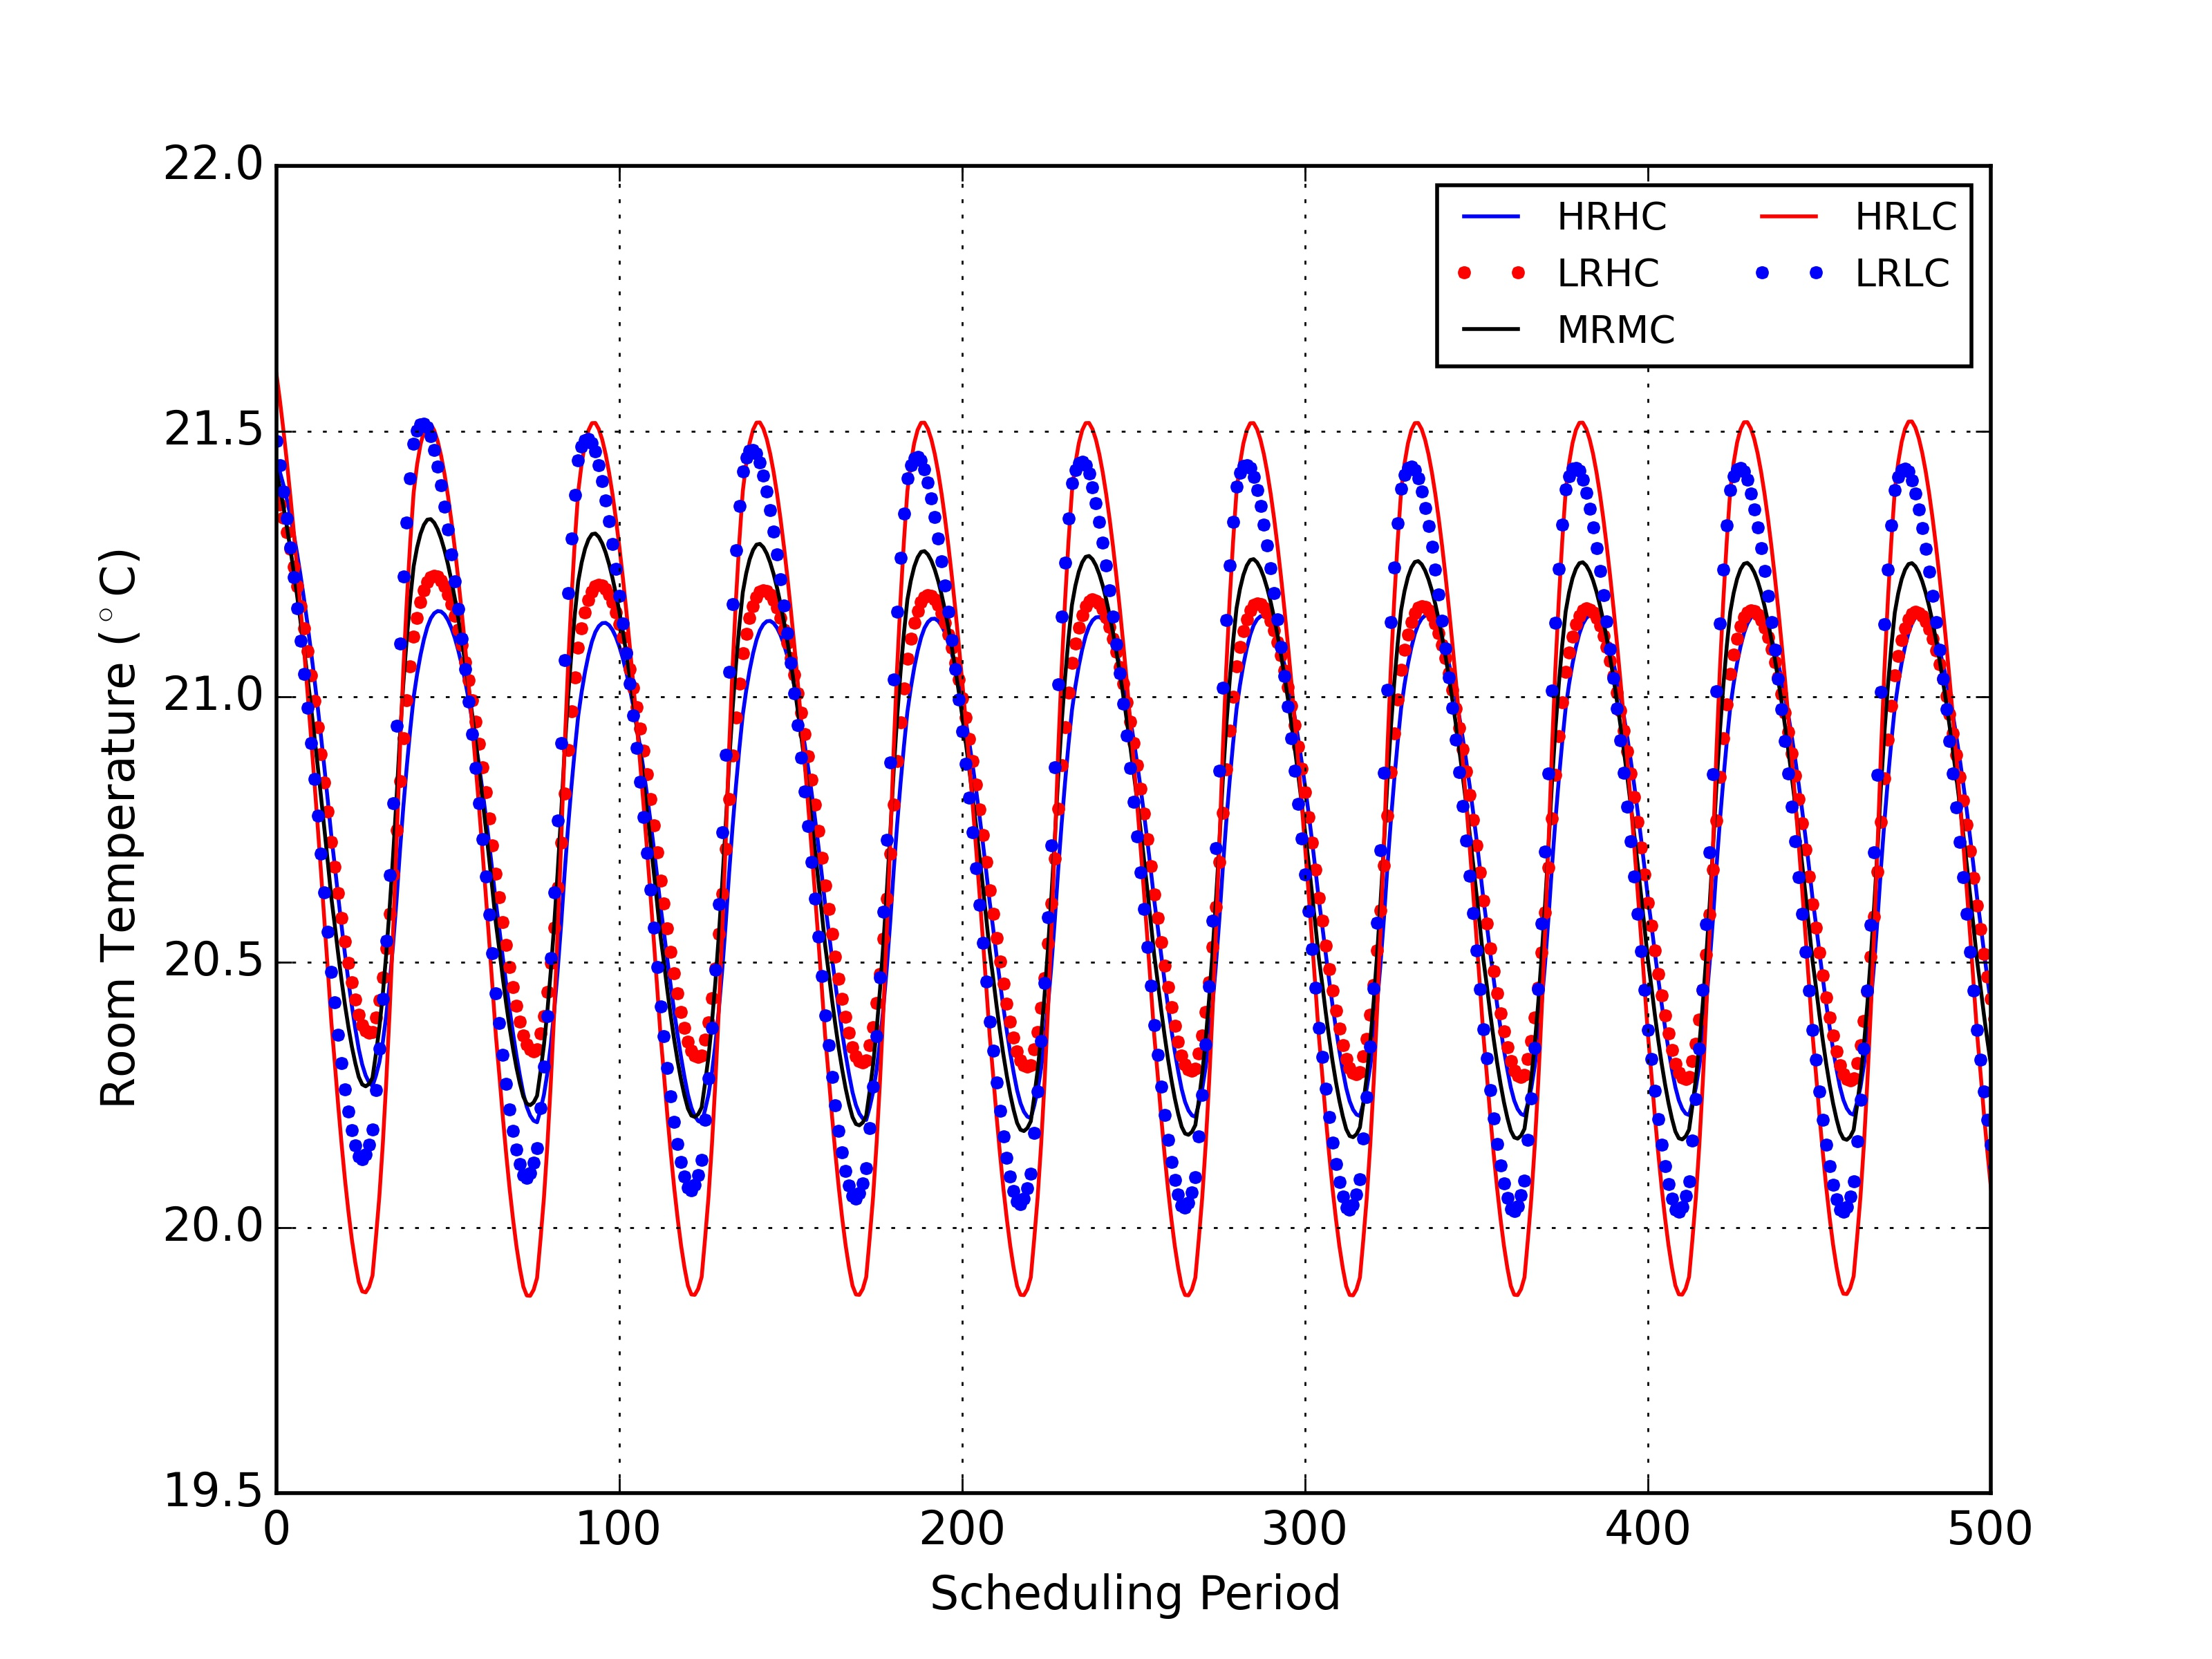
\includegraphics[width=0.74\linewidth,keepaspectratio]{./figs/mip_roomtemp.jpg}		
	\caption{Room temperature dynamics}
	\label{fig:mip_rt}
\end{figure}

Figure \ref{fig:mip_rt} illustrates the fluctuation of zone temperatures for 5 different building types, as defined in Table \ref{tab:rc_wall_win}. In this experiment, we assume that the HVAC is off and no meetings are scheduled. We simply calculate the zone temperature at each time step without optimizing any parameter. Thus, the zone temperatures are solely affected by the outdoor temperature and the solar gain. As the zones differ by a high (H), medium (M) and low (L) value for their thermal resistance (R) and capacitance (C), we observe that the temperatures at each zone fluctuate at a different scale. Some zones (eg. HRLC and LRLC) release and absorb heat at a faster rate, hence the zones' temperatures swing more drastically than other zones (eg. LRHC and HRHC). %At first, it may be seem that the latter zones are more energy efficient as the zones' temperature can be maintained at relatively smaller fluctuations, and be kept at a tighter comfort range. 
At first, it may seem that the latter zones are more energy efficient, as the zones' temperatures have relatively smaller fluctuations, and the room temperature can be kept within a tighter comfort range easily.
This is not necessarily true. The room temperatures are influenced by the diurnal temperature variation\footnote{Diurnal temperature variation is the variation between a high temperature and a low temperature that occurs during the same day.} of a location, and the energy consumption is impacted by the gap between outdoor temperature and the occupied comfort temperature range. Some building types require more energy for space heating or cooling at the beginning but they have better insulation to retain heat, whilst other building types have less insulation but are able to leverage the outdoor temperature to achieve comfort temperature for a short period of time. %require little energy  for space heating and cooling (passive house concept)
In the following, we look further into the HVAC consumption of each building types, with meetings being scheduled at different hours of a day.

\vspace{10px}
\emph{Case Study 2} \quad \textsl{How does meeting scheduling affect energy consumption at different rooms?}
\vspace{10px}

\begin{figure}
	\centering
		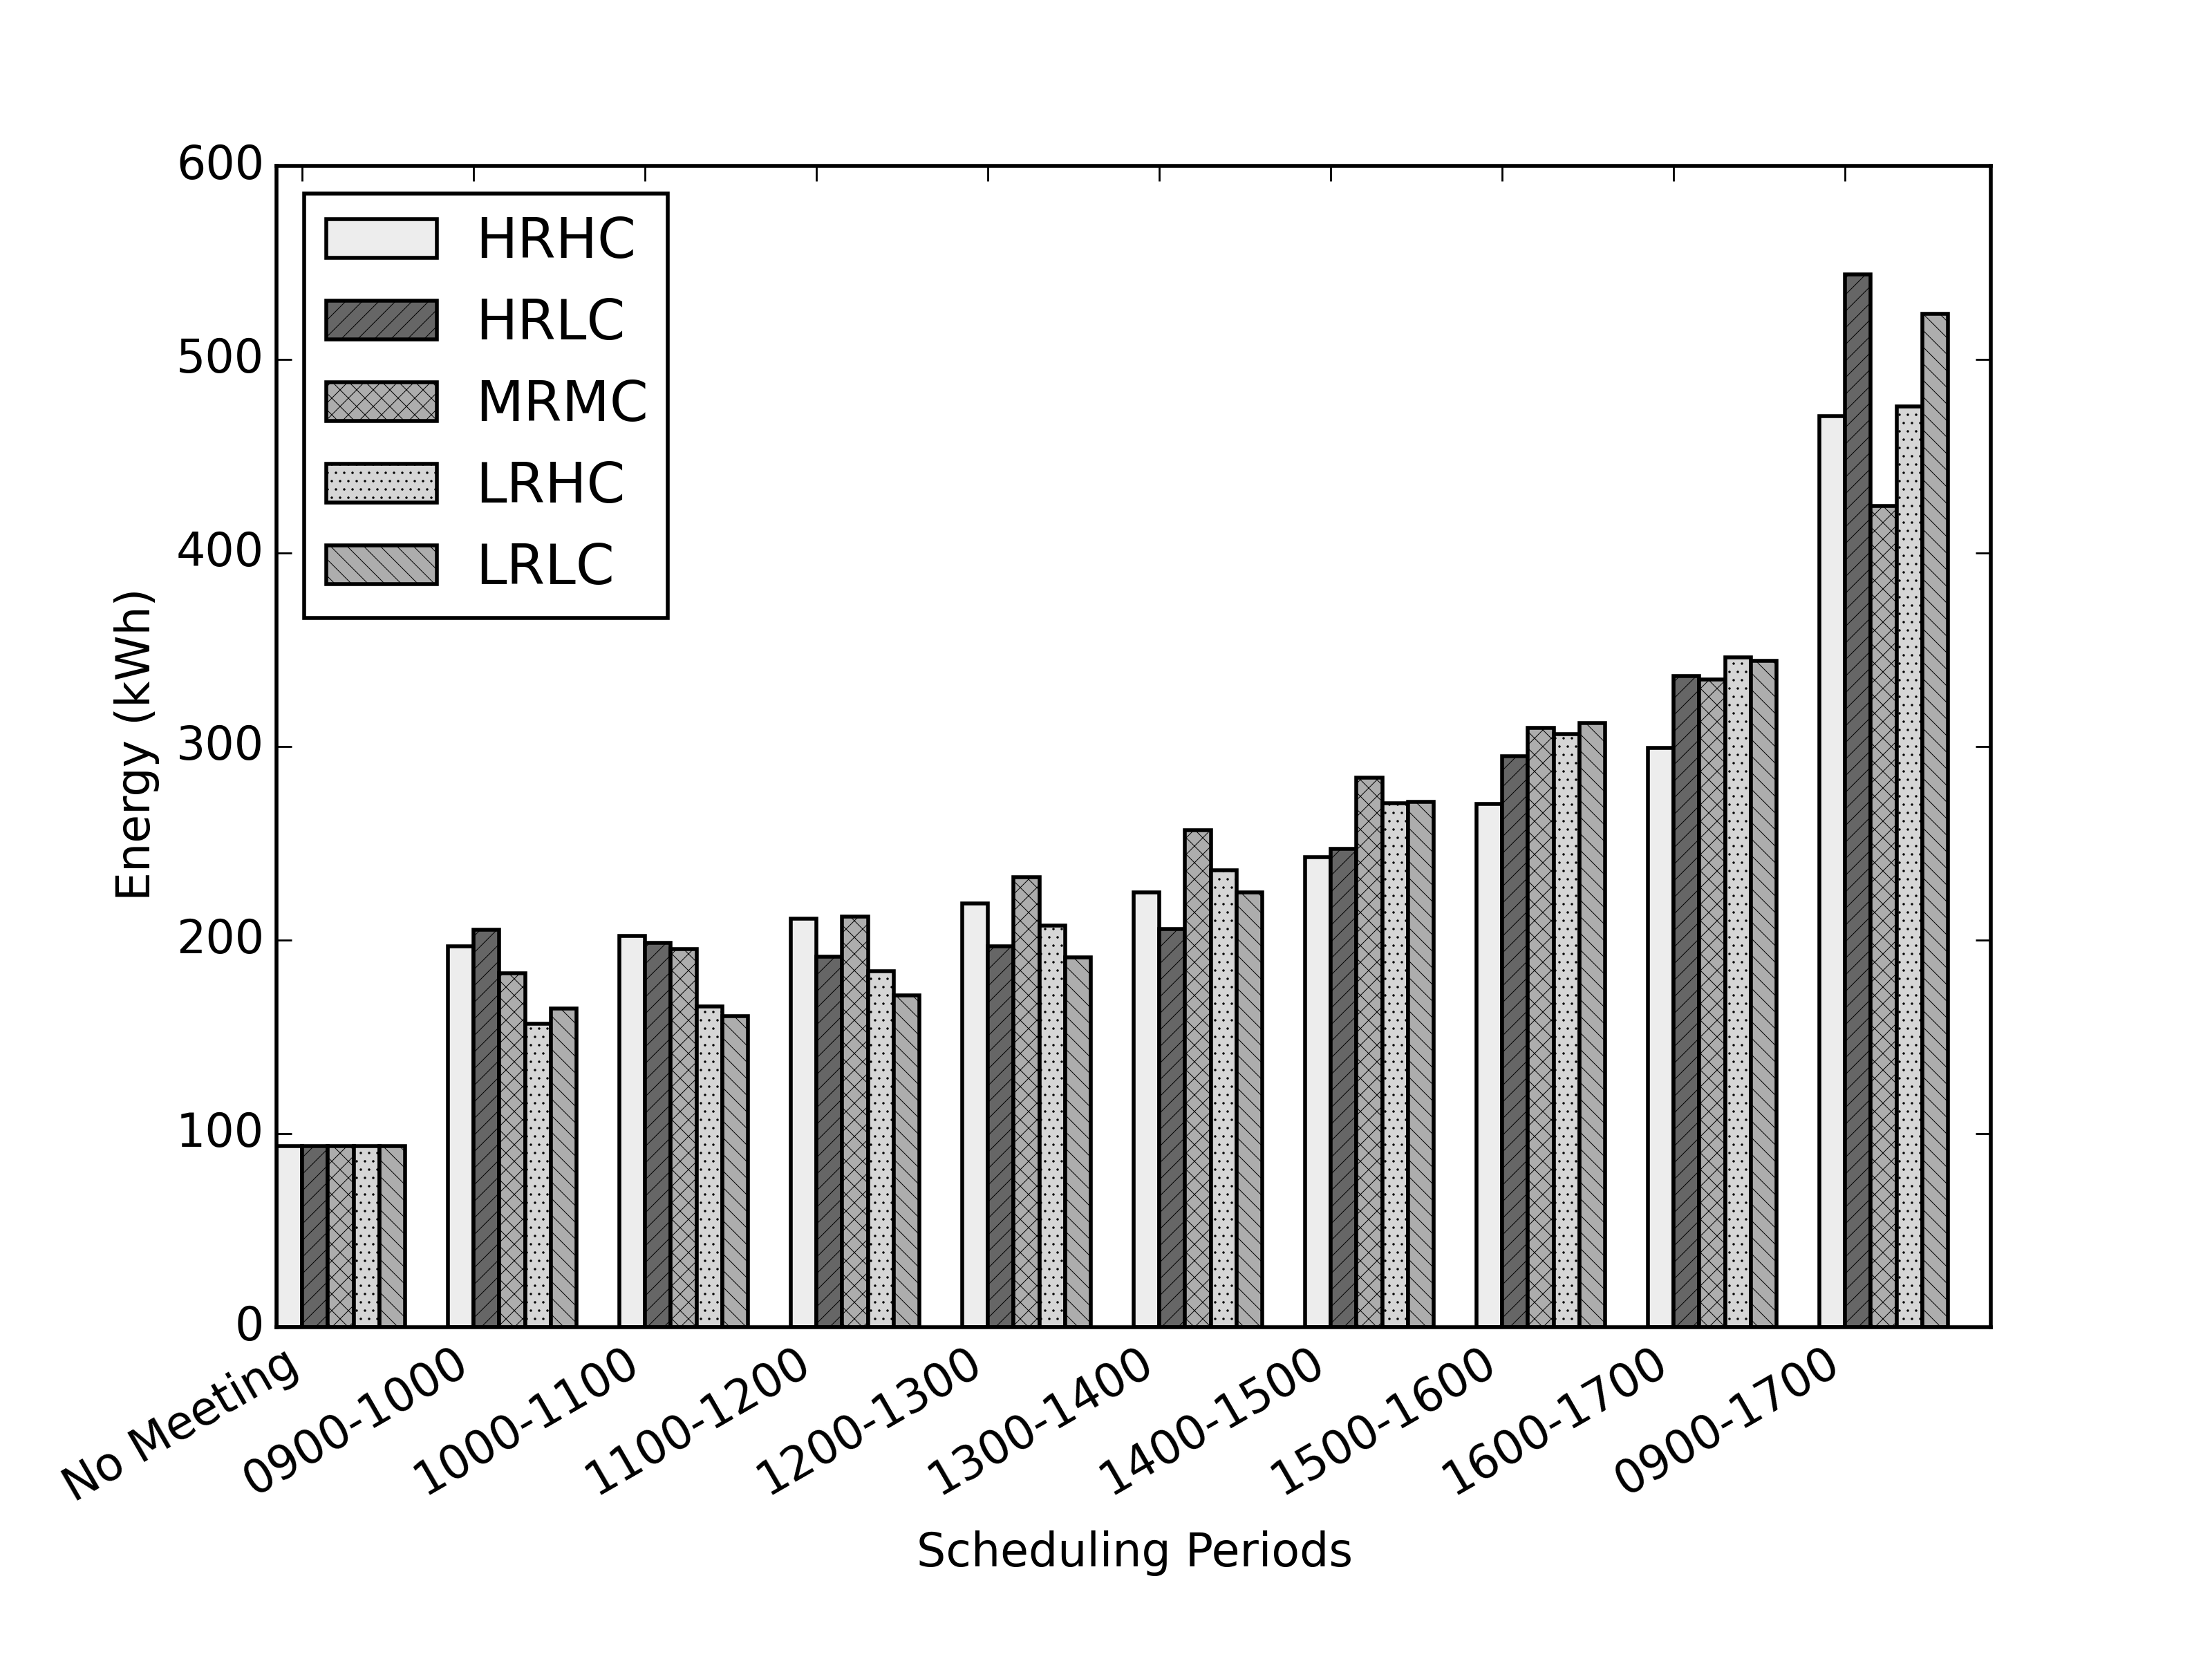
\includegraphics[width=0.74\linewidth,keepaspectratio]{./figs/mip_room_energy.png}		
	\caption{Energy consumption of different building types with meetings held at different time of the day}
	\label{fig:mip_re}
\end{figure}

Figure \ref{fig:mip_re} shows the energy consumption of 5 rooms located in different buildings, with meetings being held at different time of the day over 5 summer days. The meeting schedule is fixed, and the HVAC control is being optimized. The leftmost set of bars shows the energy consumption when no meeting is being held. The HVAC is turned on but running at a minimum load to maintain the basic ventilation standard required by \cite{ashrae2013thermal}. The rightmost set of bars shows the energy consumption when HVAC is turned on for an eight hour meeting held everyday. This setting can also be perceived as the conventional approach where HVAC is turned on throughout the day regardless of the occupancy of a zone. The rest of the graph shows the energy consumption for an hour meeting scheduled at the a given hour (e.g. 0900-1000) over 5 days. The HVAC is turned on to bring the zone temperature to 21$^\circ$C - 23$^\circ$C during occupied periods. We observe that the HVAC consumption increases when meetings are being scheduled in the evening compared to in the morning. This is due to the increase of cooling load required as the rooms get more heat gain from the sun during the afternoon and evening. However, the increase varies for different building types. The energy consumption patterns for each room type change with meetings being scheduled in the room at different hours of the day. Some consume less energy than other room types for a morning meeting, and vice versa for an evening meeting. Given various scheduling constraints, it is impossible to enumerate energy consumption patterns for all combinations of different schedules. Hence, automatic selection of room and time is crucial to identify optimal scheduling options and minimise HVAC expenses. 

\vspace{10px}
\emph{Case Study 3} \quad \textsl{Which room consumes the least amount of energy in a building?}
\vspace{10px}

\begin{figure}
	\centering
		\includegraphics[width=0.5\linewidth,keepaspectratio]{./figs/mip_roomsolar.jpg}		
	\caption{Energy consumption of 9 rooms with different facing and layout at LRHC building.}
	\label{fig:mip_rs}
\end{figure}

Next, we examine if room selection is crucial for rooms with similar thermal resistance and capacitance, and that are located in the same building. The meeting schedule is fixed, and the HVAC control is being optimized. Figure \ref{fig:mip_rs} shows the energy consumption of 9 rooms that are co-located in the same building, but with different facing and layout. With an 8-hours meeting scheduled in each room for a summer day, the results show that each room consumes a slightly different amount of energy. While a building consists of multiple rooms with similar build-up, each room has different layout and window size. They also acquire different amounts of solar gain over a day. These factors impact their HVAC consumption. Notice that the center room (C) is surrounded by four internal walls, hence it is the least impacted by the outdoor temperature and the solar gain. Its energy consumption is the highest as more HVAC intervention is required for space cooling. Meanwhile, four corner rooms (NE, SE, NW, SW) which have larger windows and larger area size of external walls consume relatively less energy compared to the two middle rooms (N,S). This result shows that selecting a room within the same building with different layout and exploiting external weather conditions can be effective to reduce energy consumption, while meeting the occupant thermal comfort requirement.

\subsection{Usefulness of Standby Mode}
\label{subsec:experiments:standby}

\begin{figure}
\begin{tabular}{c}
  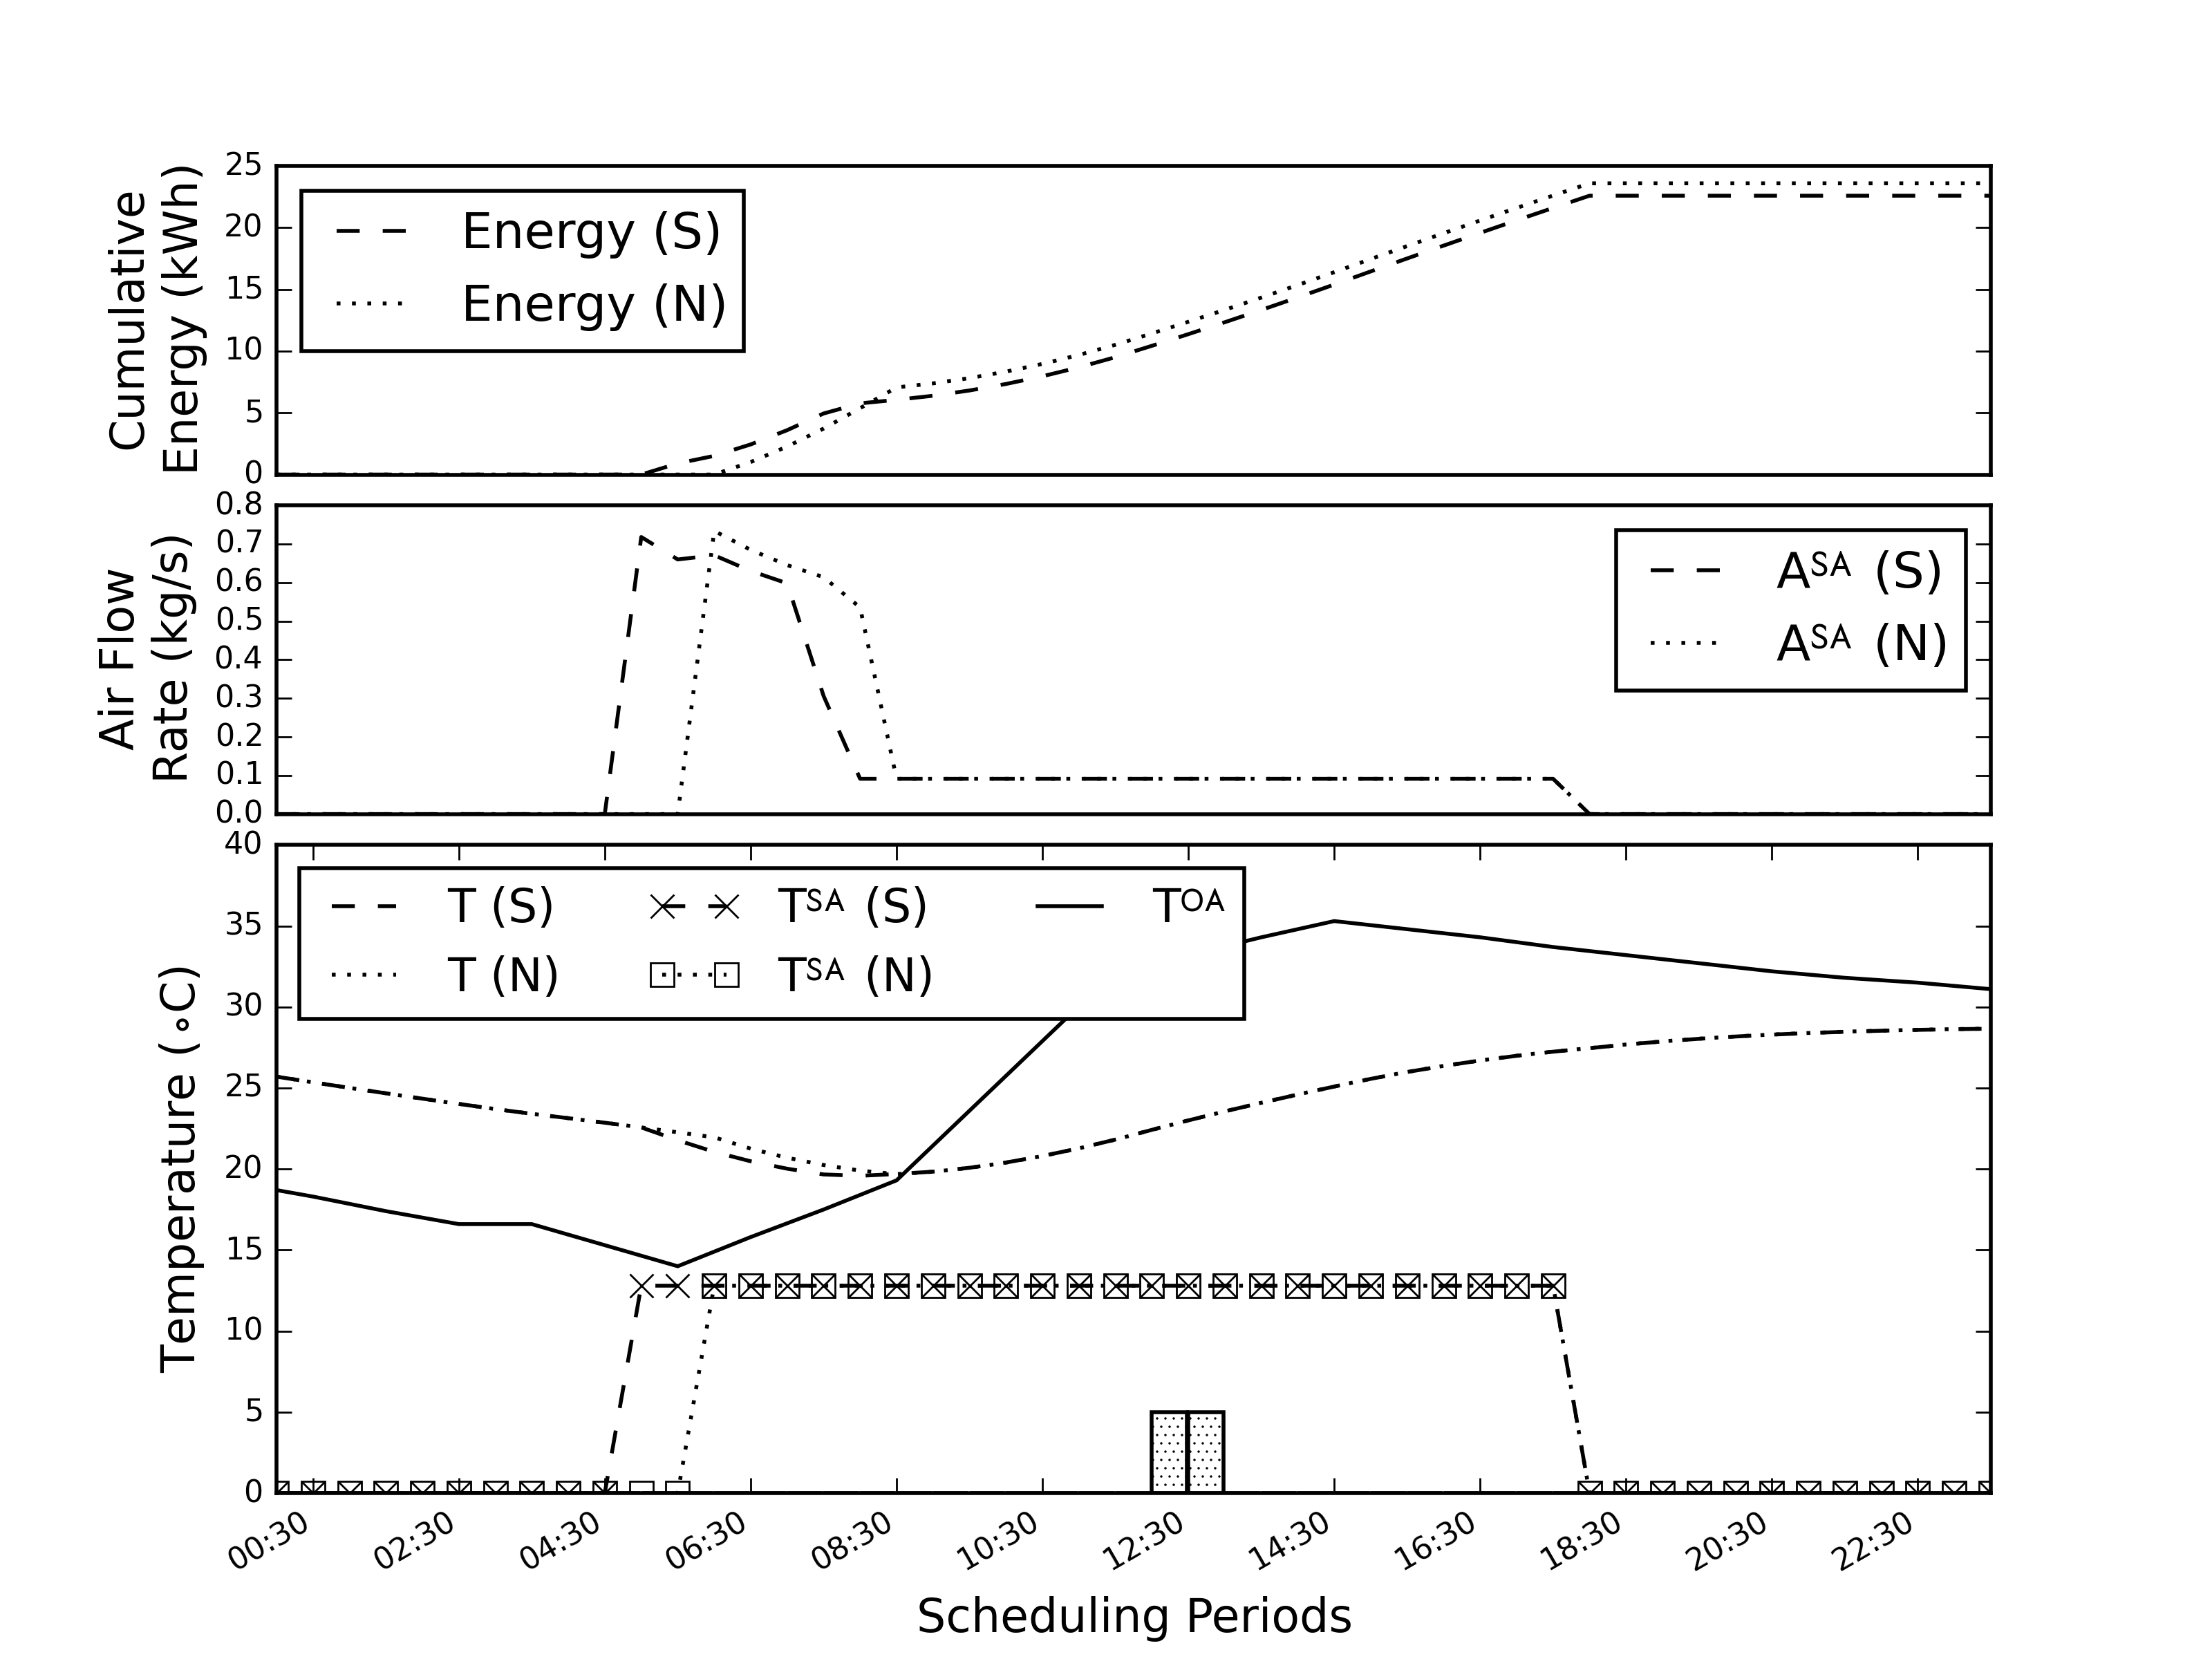
\includegraphics[width=0.9\linewidth]{figs/hrlc_opt_ws_ns_r0.png} \\
(a) HRLC \\[6pt]
  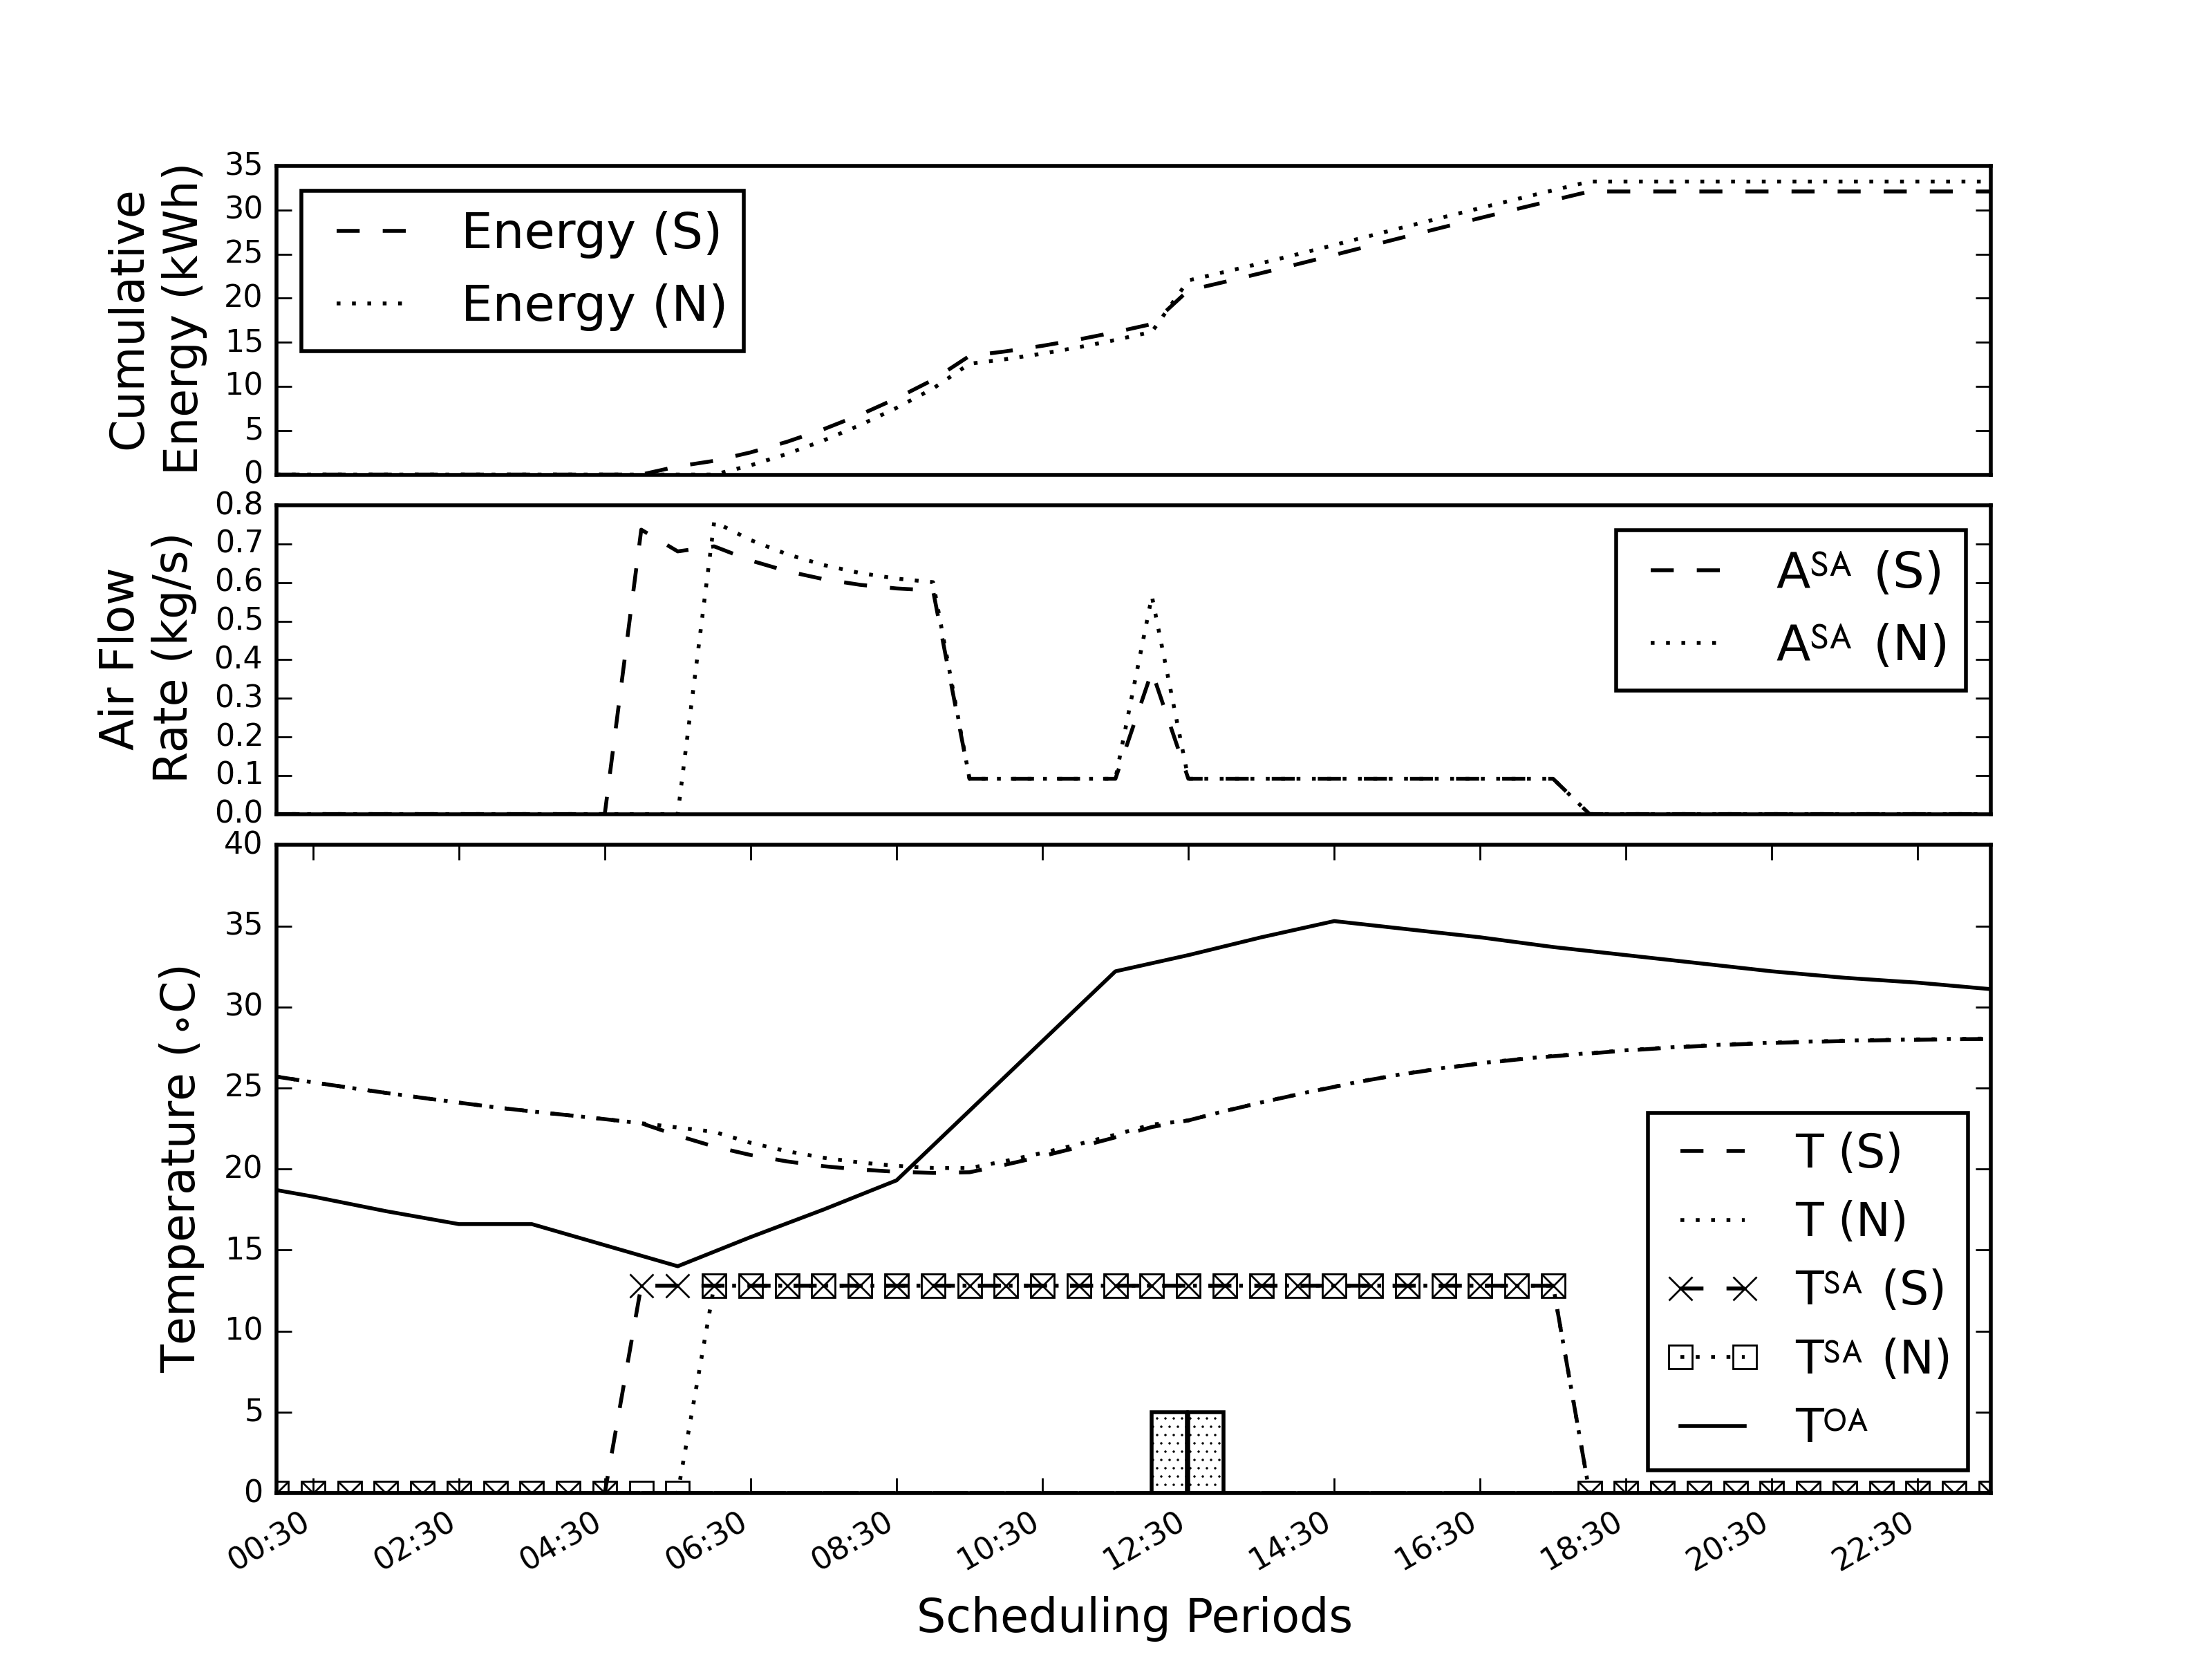
\includegraphics[width=0.9\linewidth]{figs/lrlc_opt_ws_ns_r0.png} \\
(b) LRLC \\[6pt]
\end{tabular}
\caption{HVAC control with (S) and without (N) standby mode. Our standby mode enables the HVAC to self activate outside business hours (eg. before 6 a.m.) for pre-cooling. This results in the reduction of energy consumption, compared to the HVAC control without standby mode.}
\label{fig:standby}
\end{figure}

Next we illustrate the usefulness of the standby mode. In conventional operations, HVACs are usually switched on a few hours prior to start of business (6am) and are turned off in the evening (6pm) and at night. Model predictive control strategies are capable of pre-cooling a zone, but only when the HVAC is switched on. Our standby mode enables the HVAC to self activate outside business hours to provide additional pre-cooling when this is beneficial. Because HVAC consumption is highly dependent on the temperature gap between the outdoor temperature and the conditioned air temperature, pre-cooling at night, when the outdoor air temperature is cooler, can reduce energy consumption. 
The following experiments show that such pre-cooling can be beneficial not only for early morning meetings, but also, more surprisingly, for afternoon meetings. 

Figure~\ref{fig:standby} compares the operations of the HVAC optimally controlled by the model in Section~\ref{sec:mip:control} with standby mode (S) and without standby mode (N). In this experiment, a single meeting is scheduled to occur between 12:00-13:00 in the HRLC zone and the LRLC zone of a given day. The occupied period is depicted as two vertical blocks (30 minutes each) in the third subgraph of Figure~\ref{fig:standby} (a) and (b). Observe that in the HRLC zone, when the HVAC is running with standby mode enabled, it activates as early as 05:00 and pushes between 0.72 and 0.3 kg/s of supply air at 12.8$^\circ$C to bring down the zone temperature to approximately 19$^\circ$C by 07:30. Between 04:30 and 06:00, the outdoor temperature lies between 14 and 15$^\circ$C, which is just about 1-2$^\circ$C higher than the 12.8$^\circ$C conditioned air temperature. In constrast, when the HVAC is running without the standby mode, the supply air is pushed into the room at a higher average rate between 0.73 and 0.53 kg/s right after the HVAC is turned on at 06:00, which, as the outdoor temperature is higher at that time (15-19$^\circ$C), requires a higher rate of energy consumption. During the day, the zone temperature increases slightly due to the daytime thermal gain, and at 12:00, the room temperature falls exactly within the comfort range of 21$^\circ$C - 23$^\circ$C. 

In the LRLC zone, a slightly different optimal control scheme is identified. With the standby mode enabled, the HVAC is activated at 05:00 and pushes between 0.73 and 0.58 kg/s of supply air at 12.8$^\circ$C until 09:00, where the room temperature reaches 20$^\circ$C. In contrast, with the standby mode disabled, the supply air is pushed into the room only from 06:00 to 09:00. Given that the outdoor temperature is rising, and the pre-cooling period is relatively short, it fails to bring down the room temperature further. At 12:00, when the meeting starts, the room is cooled down again. This time, the standby-mode enabled HVAC requires cooling about half the amount of supply air, which brings significant energy savings since the outside temperature is around 33$^\circ$C. 

Altogether, in both examples, the standby mode reduces consumption by 3.5-4.4\%. %(~1-2 kWh)
As shown above, a standby-mode-enabled HVAC can be effective in areas with high diurnal temperature variation.  In addition to decreasing energy consumption, it can provide pre-cooling at off-peak electricity cost. For organisations that are charged by electricity suppliers according to their peak consumption, another benefit of the standby mode is that it can help smooth the peak that is regularly observed at the start of the operating hours. We also notice that with standby mode, the scheduler is capable of generating more number of feasible solutions by reactivating the HVAC at off-peak hours in order to meet the occupied temperature bounds of an early morning meeting.


\subsection{Joint Model vs Simpler Models}
\label{subsec:experiments:integration}

Whilst the standby mode is beneficial, the much larger gains in our approach stem from the joint model: we now compare our joint model with simpler approaches representative of the existing literature on occupancy-based HVAC control and energy-aware meeting scheduling, and observe a significant energy consumption improvement.

Specifically, we consider a set of timetabling problems derived from the PATAT \cite{patat02} dataset 
%\footnote{\scriptsize{\url{http://www.or.ms.unimelb.edu.au/timetabling/}}}
and compare the optimal (O) solutions produced by the joint model in Section~\ref{sec:mip:scheduling}, with those produced by giving arbitrary (A) schedules and heuristic (H) energy-aware schedules as input to the HVAC control model in Section~\ref{sec:mip:control}. Several authors have argued that scheduling meetings back to back in as few rooms as possible is a suitable heuristic that takes advantage of thermal inertia to reduce energy consumption \citep{kwak2013tesla,majumdar2012energy,pan2012thermal}. In line with this, the heuristic we compare to, minimise the number of rooms used and the time gap between meetings in these rooms, subject to the scheduling constraints~\ref{eq:ms_every}-\ref{eq:ms_meeting}.\footnote{\cite{majumdar2012energy} observe that the single most important predictor of performance is good match between the room capacity and the size of the meetings. However this does not play a role in our experiments since all four rooms have the same capacity.} In all three cases (A,H,O), we run the HVAC control model with standby mode (S) and without it (N), resulting in six different methods labeled AN, AS, HN, HS, ON, OS, where for example, HS denotes HVAC control with standby mode using heuristic schedules. The conventional approach (CO), where HVAC is turned on from 6 a.m. to 6 p.m. daily, is used as the baseline.

\subsubsection{Insights to HVAC Controls: Joint Model vs. Heuristics-based Model}
Before presenting the results from a more comprehensive dataset, we first provide an insight into the HVAC controls produced by our joint model with standby mode (OS) versus the state-of-the-art energy-aware heuristic approach which schedules meetings back-to-back in the same room (HN). In this simple scenario, two one-hour meetings need to be scheduled between 12:00 to 14:30. Two rooms (R0, R1) are available. Both rooms are located at the LRLC zone but have different facing (room R0 is facing west and room R1 is facing east) thus they have different solar gain throughout a day. In the heuristic approach, both meetings are scheduled back-to-back in room R1.

\begin{figure}
\begin{tabular}{c}
  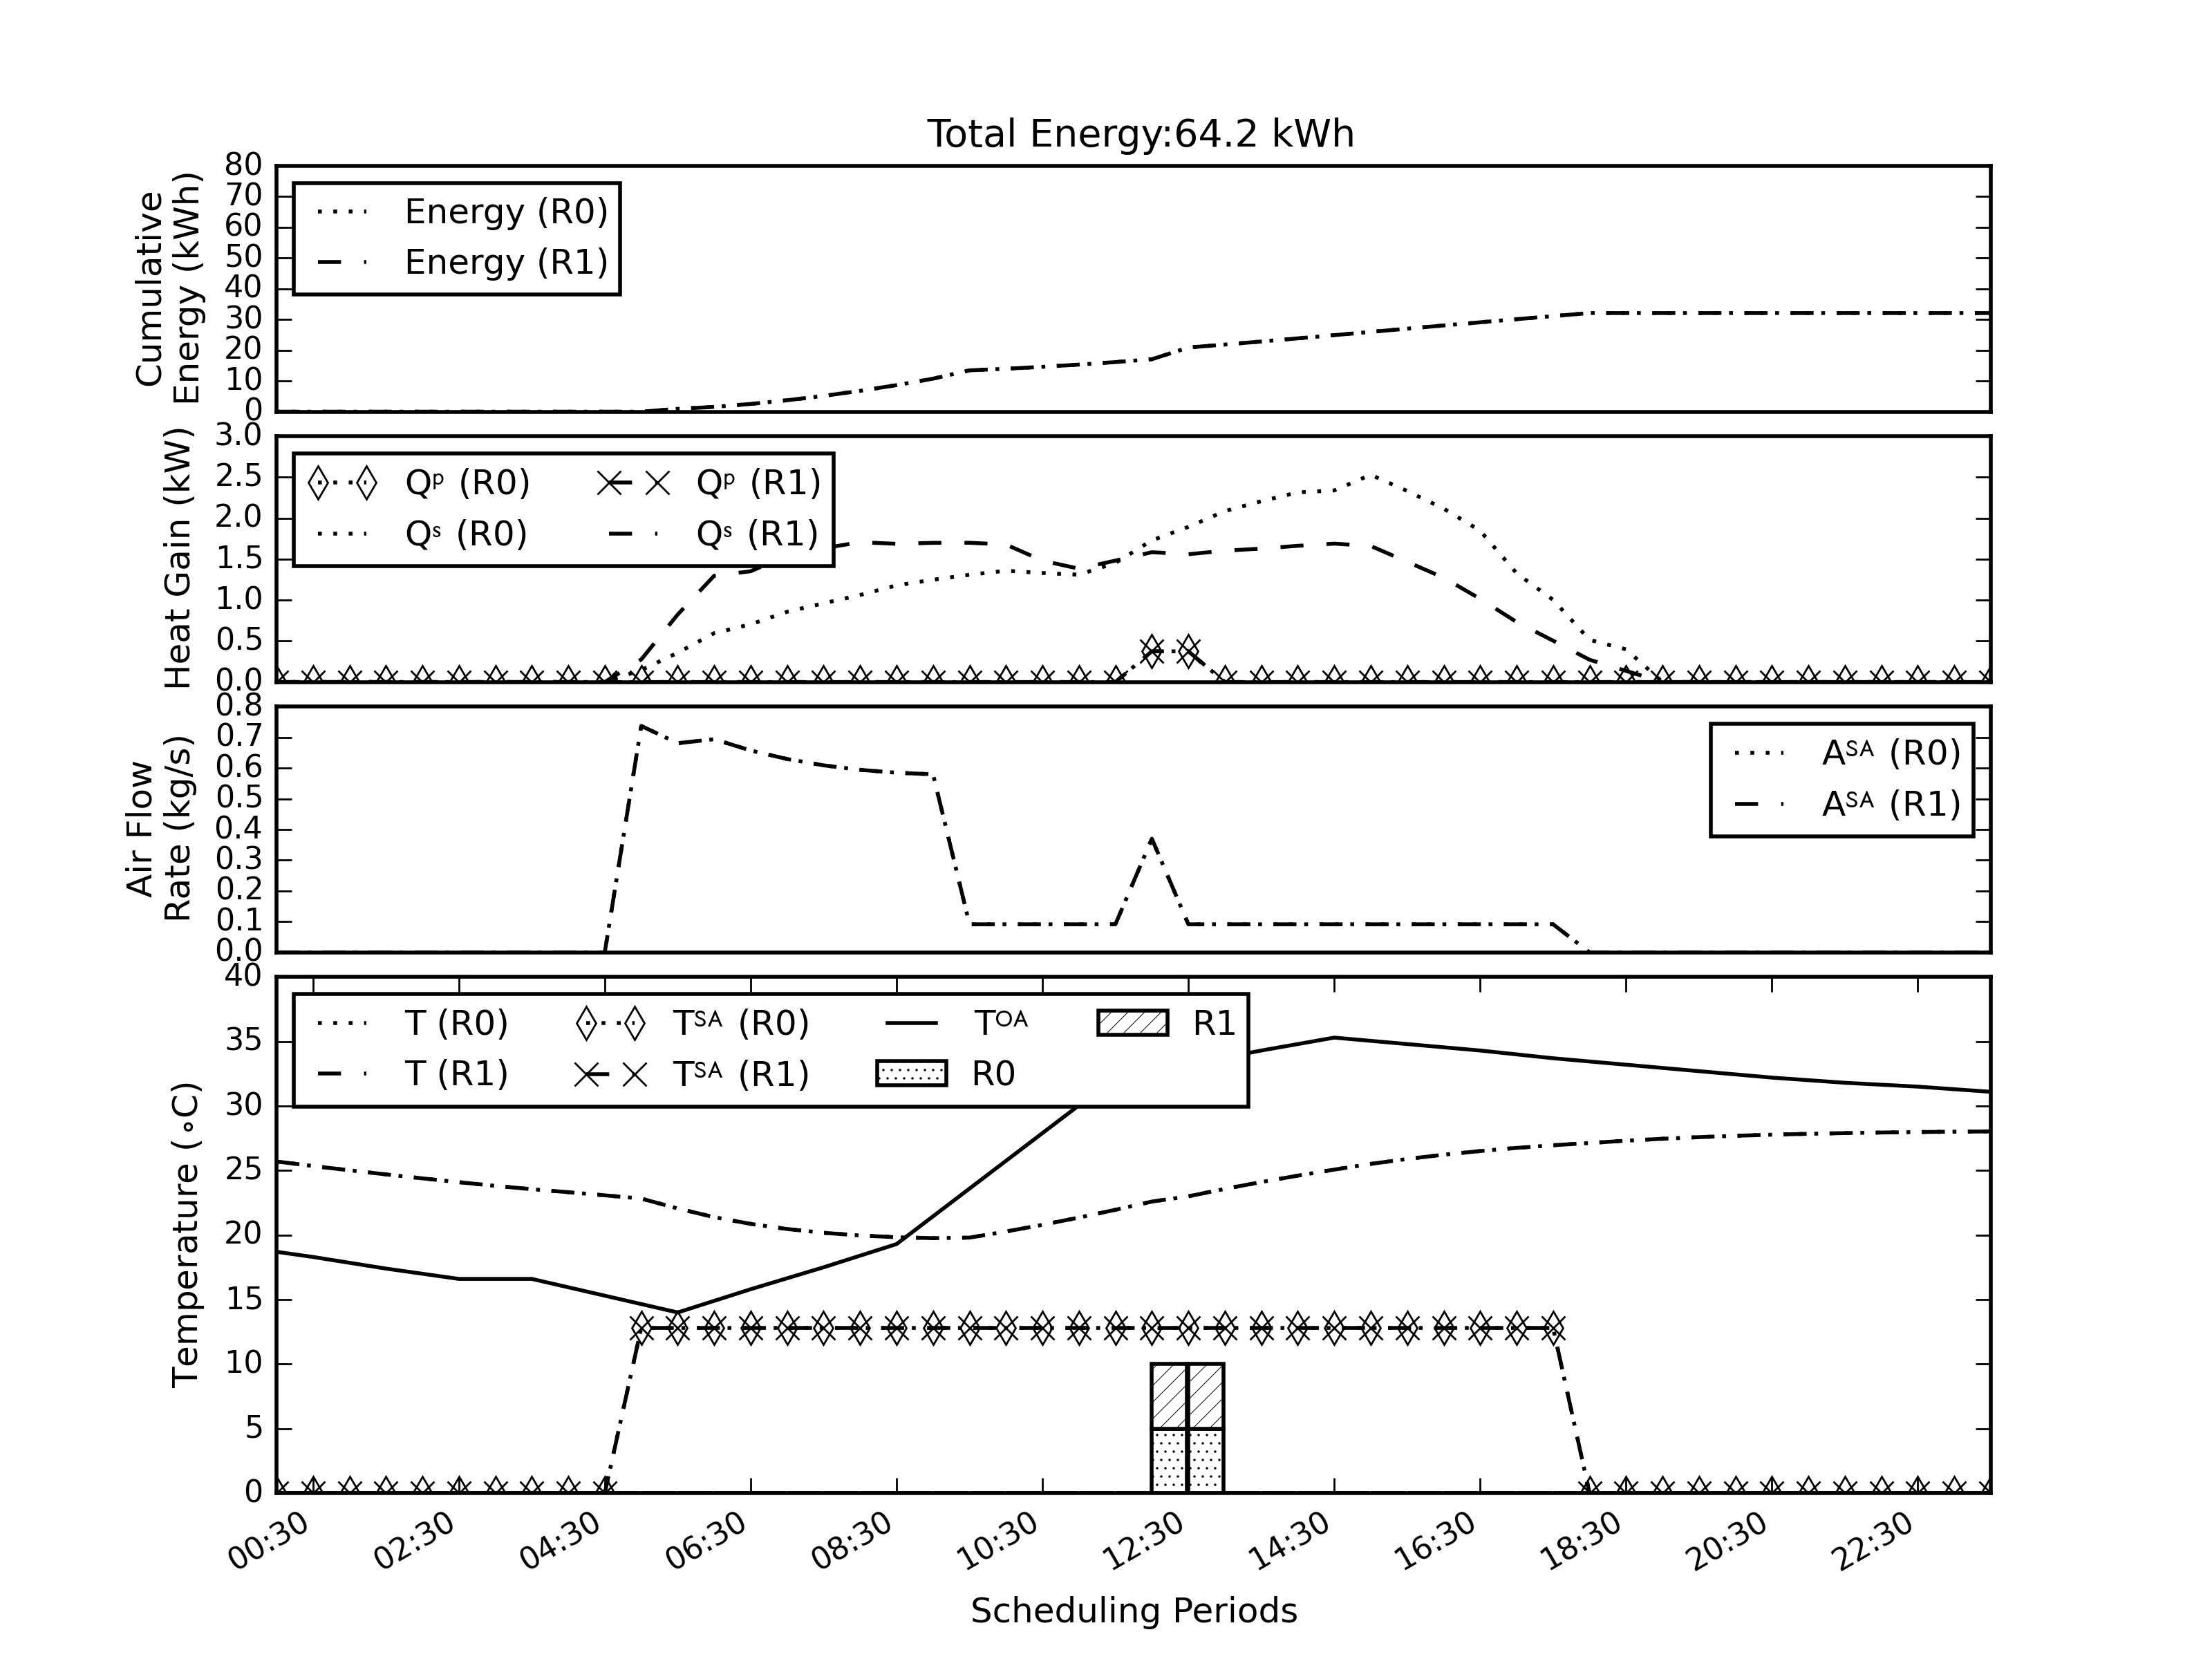
\includegraphics[width=0.9\linewidth]{figs/lrlc_opt_ws.png} \\
(a) Optimal Solution (OS) \\[6pt]
  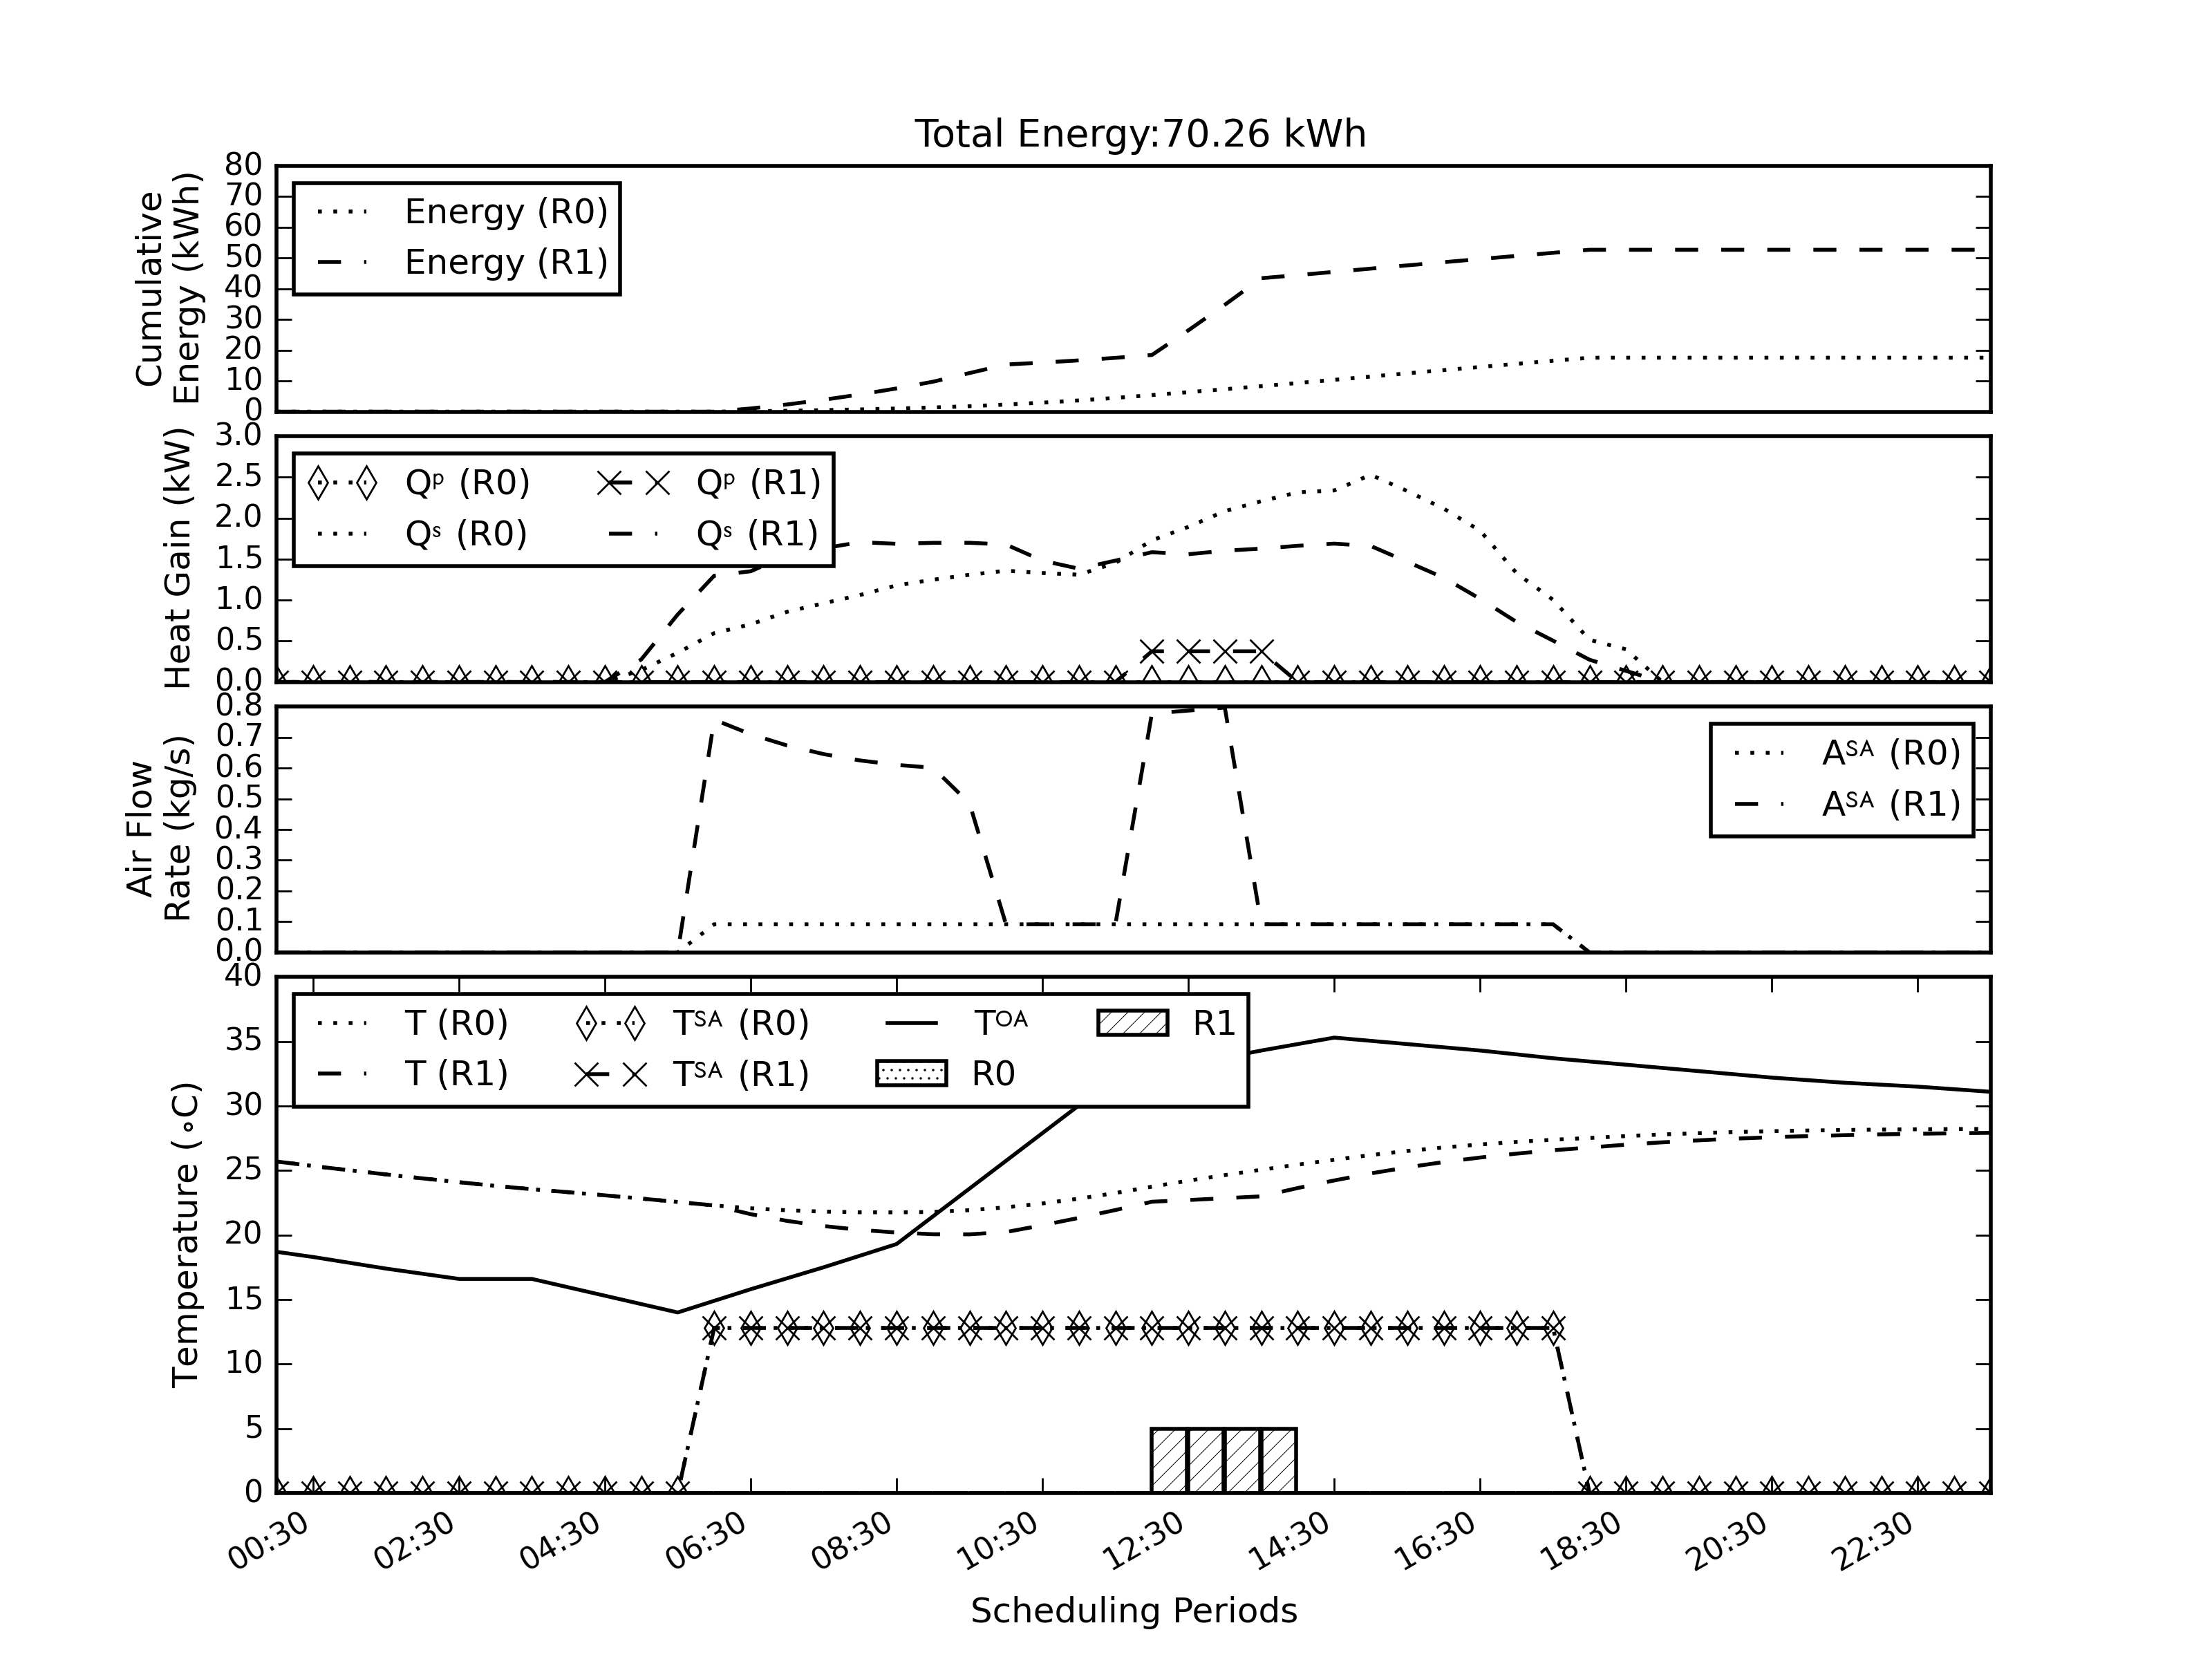
\includegraphics[width=0.9\linewidth]{figs/lrlc_b2b_ns.png} \\
(b) Back-to-back Heuristic-based Solution (HN) \\[6pt]
\end{tabular}
\caption{HVAC control with different scheduling approaches}
\label{fig:mip_scheap}
\end{figure}

Figure \ref{fig:mip_scheap} shows the results using both schemes. With our OS approach, the HVAC is turned on at 05:00 in the morning to cool down the room using the outdoor cold air. The meetings are scheduled in parallel at 12:00-13:00 as the cost of energy consumption is identified as optimal with such setting. Given both rooms being pre-cooled, the amount of outdoor air required to maintain the zones' temperature are approximately 0.36 kg/s between 12:00 to 12:30. On the other hand, using the HN approach, the HVAC is only activated at 06:00 and the meetings are forced to be scheduled in the same room. Although room R1 has been pre-cooled prior to the meetings (from 06:00 to 10:00), approximately 0.7 kg/s outdoor air are still required to be pushed into the room between 12:00 to 13:30 to maintain the zone temperature. In this simple scenario, our joint model achieves 6 kWh savings compared to the heuristic approach. We show that the heuristics of scheduling activities back-to-back in the same room in order to leverage thermal inertia does not necessary lead to energy savings.

% say thermal inertia not necessary effective
% HN: to 12.8$^\circ$C at 12:00 to 13:30 when the external temperatures are between 32$^\circ$C-34$^\circ$C.

\subsubsection{Experiment Results} 

To examine problems with different degree of constrainedness, we extracted 70 problem instances from the PATAT dataset, consisting of 
40 instances of 10 meetings each, 20 instances of 20 meetings each, and 10 instances of 50 meetings each. All meetings have up to 30 attendees, a 1.5h duration and an allowable time range of one or two random days (09:00-17:00) within the 5 days of the experiment.

The AN/AS results are obtained by selecting, for each instance, an arbitrary schedule consistent with the scheduling Constraints \eqref{eq:ms_every}-\eqref{eq:ms_meeting} in Section~\ref{sec:mip:scheduling} and using it as input to the occupancy-based HVAC control model in Section~\ref{sec:mip:control}. Similarly, the HN/HS results are obtained by selecting the schedule optimising the heuristic among those consistent with the scheduling constraints, and using it as input to the occupancy-based HVAC control model. The ON/OS results are obtained by solving the joint model for each instance.


%Conventional	522.86	Baseline	330.90
%AN	212.14	40.57	74.83
%AS	199.94	38.24	64.78
%HN	184.26	35.24	51.85
%HS	177.32	33.91	46.13
%ON	124.13	23.74	2.30
%OS	121.34	23.21	Baseline

\begin{table}[t]
\centering
\begin{tabular}{p{0.1\linewidth} p{0.25\linewidth} p{0.25\linewidth} p{0.25\linewidth}}
\hline \centering{Strategy}  & \centering{Avg. energy consumption (kWh)} &  \centering{\% Consumption vs. CO} &  \centering{\% Excess Consumption vs. OS} \tabularnewline
\hline \centering{CO}  & \centering{522.86} &  \centering{Baseline} & \centering{330.9\%} \tabularnewline
\hline \centering{AN}  & \centering{212.14} &  \centering{40.57\%} &  \centering{74.84\%}\tabularnewline
\hline \centering{AS}  & \centering{199.94} &  \centering{38.24\%} &  \centering{64.78\%}\tabularnewline
\hline \centering{HN}  & \centering{184.26} &  \centering{35.24\%} &  \centering{51.86\%}\tabularnewline
\hline \centering{HS}  & \centering{177.32} &  \centering{33.91\%} &  \centering{46.14\%}\tabularnewline
\hline \centering{ON}  & \centering{124.13} &  \centering{23.74\%} &  \centering{2.30\%}\tabularnewline
\hline \centering{OS}  & \centering{121.34} &  \centering{23.21\%} &  \centering{Baseline} \tabularnewline
\hline
\end{tabular}
	\caption{Comparison of conventional approach (CO) with arbitrary (A), heuristic (H), and optimal (O) scheduling strategies over HVAC with (S) and without (N) standby mode.}
	\label{tab:sche_e}
\end{table}

\begin{table}[t]
\centering
\begin{tabular}{p{0.1\linewidth} p{0.12\linewidth} p{0.12\linewidth} p{0.12\linewidth} p{0.12\linewidth} p{0.12\linewidth} p{0.12\linewidth}}
\hline \centering{Strategy}  & \multicolumn{3}{c}{Avg. energy consumption (kWh)} &  \multicolumn{3}{c}{\% Excess Consumption vs. OS} \tabularnewline
\hline \centering{Meetings}  & \centering{10} &  \centering{20} & \centering{50} &  \centering{10} & \centering{20} & \centering{50} \tabularnewline
\hline \centering{AN}  & \centering{163.8} & \centering{219.8} & \centering{380.0} & \centering{64\%}  & \centering{95\%} & \centering{70\%} \tabularnewline
\hline \centering{AS}  & \centering{154.2} & \centering{206.0} & \centering{361.4} & \centering{55\%}  & \centering{83\%} & \centering{62\%}\tabularnewline
\hline \centering{HN}  & \centering{142.5} & \centering{178.8} & \centering{355.6} & \centering{43\%}  & \centering{59\%} & \centering{59\%}\tabularnewline
\hline \centering{HS}  & \centering{137.8} & \centering{172.0} & \centering{340.1} & \centering{38\%}  & \centering{53\%} & \centering{52\%}\tabularnewline
\hline \centering{ON}  & \centering{100.4} & \centering{115.8} & \centering{232.8} & \centering{0.8\%} & \centering{3\%}  & \centering{4\%}\tabularnewline
\hline \centering{OS}  & \centering{99.7}  & \centering{112.5} & \centering{223.4} & \multicolumn{3}{c}{Baseline} \tabularnewline
\hline
\end{tabular}
	\caption{A detailed breakdown by meeting size using different strategies.}
	\label{tab:sche_e_breakdown}
\end{table}

Table~\ref{tab:sche_e} shows, for each of the 6 approaches, the average energy consumption per room over the 70 instances, and the percentage of consumption taking the conventional approach (CO) as the baseline. Table~\ref{tab:sche_e_breakdown} provides a detailed breakdown by meeting size. The results show a clear improvement as we move from arbitrary schedules (AN/AS), that are currently the norm with room booking systems, to energy aware schedules (HN/HS), and a much greater improvement when these  schedules take into account the capabilities of occupancy-based HVAC control (ON/OS). Specifically, the ON/OS approaches consume only 23\% of the conventional approach, and are 50\%-70\% better than the state-of-the-art approaches. The interactions between the various scheduling constraints, the thermal dynamics of the building and the HVAC control are so complex that heuristic methods can only achieve a fraction  of the performance of the global optimisation methods enabled by our MILP model.  As expected, the gain conferred by the standby mode  decreases as we move to schedules that make better time and location decisions. Similarly, we observed that for more constrained problems (e.g. with 50 meetings), the standby mode is more effective, because there is a greater likelihood that meetings need to be scheduled in rooms that require higher cooling load which the standby mode can mitigate by pre-cooling.


\section{Related Work}
\label{sec:mip:related}

Occupancy information, knowing whether or not there are people in a room and ideally also knowing how many people there are in a room, is at the basis of moving away from schedule-based control towards occupancy-based control. Schedule-based control is inefficient as it operates HVAC systems according to a fixed schedule that often assumes maximum zone occupancy. Occupancy-based control, on the other hand, uses MPC approach and optimises HVAC control based on the detected or forecast occupancy information. \cite{klein2012coordinating} and \cite{oldewurtel2012use} take into account occupancy forecasts and weather to estimate energy saving opportunities. \cite{goyal2013occupancy} also take into account occupancy forecasts and compare the performance of MPC strategies with feedback controllers using occupancy measurements. \cite{mady2011stochastic} build occupancy model and use MPC to improve on energy efficiency while maximising occupant comfort. \cite{mamidi2012adaptive}, \cite{li2012measuring}, \cite{erickson2009energy} and \cite{agarwal2010occupancy} deploy sensors to detect real-time occupancy and use this information to control HVAC system in an adaptive manner. These previous works on occupancy-based HVAC control, also including works by \cite{brooks2015energy,mady2011stochastic,parisio2013randomized,xu2009model}, treat occupancy information as an input parameter and not as a control variable. Our work is different as it incorporates both HVAC control and occupancy scheduling into a unified model. In addition, our standby mode improves the feasibility and solution quality of model-predictive HVAC control methods. It is worth noting that the work on sensor-based occupancy detection approach complements our work, in which the detected occupancy information can be taken as an additional input into our model to reflect the actual occupancy flow in the buildings. 

%Their conclusion is that occupancy predictions can lead to additional energy savings over occupancy measurements especially when ventilation standards change. Currently the ASHRAE ventilation standard \cite{ashrae} requires that a certain amount of outside air is mixed with return air from the zones regardless whether a zone is occupied or not.

Various methods have been used to solve the non-linear non-convex optimisation problem in HVAC control. In \cite{klein2012coordinating}, the HVAC control is simplified to a linear model by assuming the supply air temperature is constant, thus forming a linear function to calculate only the supply air flow rate. \cite{oldewurtel2013importance} consider rather complex HVAC actuation including the control of blind positions, lighting, chiller, cooling tower, radiators etc. They apply sequential linear programming using MAP (Method of Approximation) programming \citep{griffith1961nonlinear} to linearise their HVAC model. \cite{ma2011distributed} solve the non-linear HVAC control constraints using dual decomposition and \cite{sun2010integrated} adopt lagrangian relaxation and dynamic programming using surrogate subgradient method. Some works \citep{wang2000model, xu2009model, mossolly2009optimal} implement genetic algorithms to search for optimal value of the supply air temperature and flow rate. In our work, we use McCormick's relaxation that guarantees to return an optimal lower bound on the objective function. The need to reduce computational effort and scalability of the joint model are our motivating factor to develop a linearised model for HVAC control. 

Much of the existing literature on energy-aware scheduling methods typically take advantage of thermal inertia using heuristics such as minimising the number of rooms used and/or assigning lower costs to meetings scheduled back to back in the same room \citep{pan2012thermal,kwak2013tesla,majumdar2012energy,chai2014minimizing}. An important limit of these works is that they all share a black-box modeling approach for calculating HVAC energy consumption. This black-box approach confines the search to a rather limited space that does not exploit the HVAC's full capabilities. Another limitation is the assumption of an anonymous list of meeting participants, which ignores the existence of meeting conflicts and the fundamental need for resolving them. 

\cite{kwak2013tesla} analyse the impact of scheduling flexibility on energy savings, based on the historical data of a conventional HVAC control approach. Although we have not quantified explicitly, our experiments suggest that occupancy-based HVAC control helps to mitigate the impact of less flexible scheduling requests. However, in future, it would be interesting to study the tradeoff between scheduling flexibility versus HVAC control. For example, with occupancy-based control, what is the minimum scheduling flexibility required to achieve the same energy savings, compared to conventional HVAC control with some scheduling flexibility? Such study is interesting as it allows us to quantify the difference in terms of energy gain, given the ability to manipulate the HVAC operations, the flexibility to schedule meeting requests, or both.

There has been a significant amount of work that focuses on meeting scheduling \citep{modi2004multiagent,refanidis2010constraint,tran2016smart} and timetabling \citep{merlot2002hybrid,di2002multi,abdullah2007tabu}. Our work differs from these established field by adding an additional objective to conserve energy in the buildings where these activities are held. 

Energy-oriented scheduling has gained more attention in recent years due to the significant cost saving opportunities. 
\cite{ifrim2012properties} present a MIP-based energy-price savings scheduling model to reduce cost in production scheduling. \cite{dupont2012energy} use CP to develop an energy aware framework for virtual machine placement in cloud-based data centers. \cite{scott2013residential} describe an online stochastic MILP to schedule home appliances based on real-time pricing. \cite{ono2012risk} develop a HVAC control approach that integrates with occupant activities scheduling and blind control in a smart home.  Most works focus on energy-aware scheduling in production lines, data centers and residential buildings whilst our work specifically targets energy-efficient scheduling in commercial offices and university buildings, where HVAC consumption dominates the building's energy consumption. 



\section{Conclusion and Future Work}
\label{sec:mip:conclusion}

In this work we focus on meeting scheduling, as meeting scheduling is one practical approach to strategically control occupancy flows and optimise HVAC utilisation. However, our model is more broadly applicable to scheduling occupant activities within specified time windows, and ultimately, can be integrated into a range of room booking and scheduling systems. To bring awareness of the capabilities of the building's HVAC system to the scheduling process, we solve a joint HVAC control and occupancy scheduling problem. This problem involves determining the times and locations of a set of meetings, as well as the supply air temperature and air flow rate for  each building zone, so as to minimise HVAC consumption. Existing approaches solve the HVAC control problem and the occupancy scheduling problem in isolation. While the joint problem is more challenging, it does achieve a much higher rate of energy savings. 

Directions for future work include extending our model to include more HVAC parameters such as humidity, return air ratio, damper control and conditioned air temperature. This involves the modeling of chiller and boiler operations on the supply side of the HVAC system. A more comprehensive HVAC model helps to improve the accuracy of HVAC control and the prediction of energy consumption in buildings. In addition, further research is needed to learn and improve the building thermal dynamics model using real data. Specifically, the RC parameters can be calibrated based on temperature data collected from actual buildings using machine learning techniques. 

We are also interested in exploring the CP formulation of joint HVAC control and meeting scheduling. As the joint model consists of hybrid discrete-continuous variables, we will reformulate it by discretizing the HVAC control variables, and compare the solution quality generated by both MIP and CP models. 

%In the coming chapters, we show how our joint model can be scaled to solve larger problems and handle impromptu meeting requests in real-time.


% - Warm start NLP with LP model?


%These equations form a system of nonconvex non-linear constraints, which constitute a challenge when embedded in optimisation problems. convex quadratic relaxation of the HVAC control equations that is easily embedded in MIP.

%Adding humidity --> 
%Multilinear expressions have been extensively studied in
%the literature and corresponding convex envelopes are well-defined in some
%cases. For bilinear expressions, convex envelopes were introduced by McCormick
%in [37,4] (Figures 2(a) and 2(b)) Multilinear terms such as vivjvk are relaxed
%using a sequential bilinear approach. The trilinear envelopes introduced by [38,
%39] were also considered. Nevertheless, on all applications of interest, numerical
%experiments have shown that the sequential McCormick relaxation offers
%comparably tight bounds.





